\documentclass[twoside]{book}

% Packages required by doxygen
\usepackage{calc}
\usepackage{doxygen}
\usepackage{graphicx}
\usepackage[utf8]{inputenc}
\usepackage{makeidx}
\usepackage{multicol}
\usepackage{multirow}
\usepackage{textcomp}
\usepackage[table]{xcolor}

% NLS support packages
\usepackage{polski}
\usepackage[T1]{fontenc}

% Font selection
\usepackage[T1]{fontenc}
\usepackage{mathptmx}
\usepackage[scaled=.90]{helvet}
\usepackage{courier}
\usepackage{amssymb}
\usepackage{sectsty}
\renewcommand{\familydefault}{\sfdefault}
\allsectionsfont{%
  \fontseries{bc}\selectfont%
  \color{darkgray}%
}
\renewcommand{\DoxyLabelFont}{%
  \fontseries{bc}\selectfont%
  \color{darkgray}%
}

% Page & text layout
\usepackage{geometry}
\geometry{%
  a4paper,%
  top=2.5cm,%
  bottom=2.5cm,%
  left=2.5cm,%
  right=2.5cm%
}
\tolerance=750
\hfuzz=15pt
\hbadness=750
\setlength{\emergencystretch}{15pt}
\setlength{\parindent}{0cm}
\setlength{\parskip}{0.2cm}
\makeatletter
\renewcommand{\paragraph}{%
  \@startsection{paragraph}{4}{0ex}{-1.0ex}{1.0ex}{%
    \normalfont\normalsize\bfseries\SS@parafont%
  }%
}
\renewcommand{\subparagraph}{%
  \@startsection{subparagraph}{5}{0ex}{-1.0ex}{1.0ex}{%
    \normalfont\normalsize\bfseries\SS@subparafont%
  }%
}
\makeatother

% Headers & footers
\usepackage{fancyhdr}
\pagestyle{fancyplain}
\fancyhead[LE]{\fancyplain{}{\bfseries\thepage}}
\fancyhead[CE]{\fancyplain{}{}}
\fancyhead[RE]{\fancyplain{}{\bfseries\leftmark}}
\fancyhead[LO]{\fancyplain{}{\bfseries\rightmark}}
\fancyhead[CO]{\fancyplain{}{}}
\fancyhead[RO]{\fancyplain{}{\bfseries\thepage}}
\fancyfoot[LE]{\fancyplain{}{}}
\fancyfoot[CE]{\fancyplain{}{}}
\fancyfoot[RE]{\fancyplain{}{\bfseries\scriptsize Wygenerowano Śr, 29 kwi 2015 23\-:12\-:25 dla L\-A\-B5 programem Doxygen }}
\fancyfoot[LO]{\fancyplain{}{\bfseries\scriptsize Wygenerowano Śr, 29 kwi 2015 23\-:12\-:25 dla L\-A\-B5 programem Doxygen }}
\fancyfoot[CO]{\fancyplain{}{}}
\fancyfoot[RO]{\fancyplain{}{}}
\renewcommand{\footrulewidth}{0.4pt}
\renewcommand{\chaptermark}[1]{%
  \markboth{#1}{}%
}
\renewcommand{\sectionmark}[1]{%
  \markright{\thesection\ #1}%
}

% Indices & bibliography
\usepackage{natbib}
\usepackage[titles]{tocloft}
\setcounter{tocdepth}{3}
\setcounter{secnumdepth}{5}
\makeindex

% Custom commands
\newcommand{\clearemptydoublepage}{%
  \newpage{\pagestyle{empty}\cleardoublepage}%
}


%===== C O N T E N T S =====

\begin{document}

% Titlepage & ToC
\pagenumbering{roman}
\begin{titlepage}
\vspace*{7cm}
\begin{center}%
{\Large L\-A\-B5 \\[1ex]\large 0.\-1 }\\
\vspace*{1cm}
{\large Wygenerowano przez Doxygen 1.8.6}\\
\vspace*{0.5cm}
{\small Śr, 29 kwi 2015 23:12:25}\\
\end{center}
\end{titlepage}
\clearemptydoublepage
\tableofcontents
\clearemptydoublepage
\pagenumbering{arabic}

%--- Begin generated contents ---
\chapter{Indeks klas}
\section{Lista klas}
Tutaj znajdują się klasy, struktury, unie i interfejsy wraz z ich krótkimi opisami\-:\begin{DoxyCompactList}
\item\contentsline{section}{{\bf Benchmark$<$ T $>$} }{\pageref{class_benchmark}}{}
\item\contentsline{section}{{\bf Kolejka$<$ T $>$} \\*Klasa \doxyref{Kolejka}{str.}{class_kolejka} sluzy do wykonywania podstawowych operacji na Kolejce\-: dodaj,odejmij element. Przechowuje informacje o ilosci wszysktich elementow }{\pageref{class_kolejka}}{}
\item\contentsline{section}{{\bf List$<$ T $>$} \\*Klasa \doxyref{List}{str.}{class_list} sluzy do wykonywania podstawowych operacji na Liscie\-: dodaj,odejmij element. Przechowuje informacje o ilosci wszysktich elementow }{\pageref{class_list}}{}
\item\contentsline{section}{{\bf Node$<$ T $>$} }{\pageref{struct_node}}{}
\item\contentsline{section}{{\bf Node\-L$<$ T $>$} }{\pageref{struct_node_l}}{}
\item\contentsline{section}{{\bf Node\-T$<$ Klucz, T $>$} }{\pageref{class_node_t}}{}
\item\contentsline{section}{{\bf Stack$<$ T $>$} }{\pageref{class_stack}}{}
\item\contentsline{section}{{\bf Tablica\-Asocjacyjna} }{\pageref{class_tablica_asocjacyjna}}{}
\end{DoxyCompactList}

\chapter{Indeks plików}
\section{Lista plików}
Tutaj znajduje się lista wszystkich plików z ich krótkimi opisami\-:\begin{DoxyCompactList}
\item\contentsline{section}{{\bf Benchmark.\-hh} \\*Klasa \doxyref{Benchmark}{str.}{class_benchmark} sluzy do przechowywania wynikow zlozonosci obliczeniowej i danych wejsciowych,generowania liczb rozkladu Gaussowego }{\pageref{_benchmark_8hh}}{}
\item\contentsline{section}{{\bf Kolejka.\-hh} \\*Struktura przechowujaca wartosc wezla i wskaznik na nastepny element typu \doxyref{Node}{str.}{struct_node} }{\pageref{_kolejka_8hh}}{}
\item\contentsline{section}{{\bf Lista.\-hh} \\*Struktura przechowujaca wartosc wezla i wskaznik na nastepny element typu \doxyref{Node}{str.}{struct_node} }{\pageref{_lista_8hh}}{}
\item\contentsline{section}{{\bf main.\-cpp} }{\pageref{main_8cpp}}{}
\item\contentsline{section}{{\bf main3.\-cpp} }{\pageref{main3_8cpp}}{}
\item\contentsline{section}{{\bf Operacje\-Na\-Plikach.\-hh} }{\pageref{_operacje_na_plikach_8hh}}{}
\item\contentsline{section}{{\bf Sortowanie.\-cpp} }{\pageref{_sortowanie_8cpp}}{}
\item\contentsline{section}{{\bf Sortowanie.\-hh} }{\pageref{_sortowanie_8hh}}{}
\item\contentsline{section}{{\bf Stack.\-hh} \\*Klasa \doxyref{Stack}{str.}{class_stack} sluzy do przechowywania, dodawania,zdejmowania kolejnych elementow stosu }{\pageref{_stack_8hh}}{}
\item\contentsline{section}{{\bf Struktury.\-hh} }{\pageref{_struktury_8hh}}{}
\item\contentsline{section}{{\bf Zapisz\-Stos\-Kolejka\-Lista.\-cpp} }{\pageref{_zapisz_stos_kolejka_lista_8cpp}}{}
\item\contentsline{section}{{\bf Zapisz\-Stos\-Kolejka\-Lista.\-hh} }{\pageref{_zapisz_stos_kolejka_lista_8hh}}{}
\end{DoxyCompactList}

\chapter{Dokumentacja klas}
\section{Dokumentacja klasy Benchmark}
\label{class_benchmark}\index{Benchmark@{Benchmark}}


{\ttfamily \#include $<$Benchmark.\-hh$>$}

\subsection*{Metody publiczne}
\begin{DoxyCompactItemize}
\item 
{\bf Benchmark} ()
\item 
{\bf Benchmark} (int roz, unsigned long int max)
\item 
{\bf $\sim$\-Benchmark} ()
\item 
void {\bf Ustal\-Rozmiar\-Tablicy\-Zlozonosci\-Obliczeniowej} (int roz)
\item 
std\-::ostream \& {\bf Generuj\-Liczby\-Zmiennoprzecinkowe} (long int {\bf rozmiar}, std\-::ostream \&strum)
\item 
void {\bf Transformacja\-Boxa\-\_\-\-Mullera} (float a[$\,$])
\item 
void {\bf Stworz\-Liczby\-Odniesienia} (int p[$\,$], int ile)
\item 
void {\bf Testuj} (int Ilosc\-Powtorzen, int Max\-Ilosc\-Danych, void($\ast$wsk\-\_\-fun)(double $\ast$, int))
\item 
std\-::ostream \& {\bf Zapisz\-Wyniki\-Zlozonosci\-Obliczeniowej} (std\-::ostream \&Strm, int roz)
\end{DoxyCompactItemize}
\subsection*{Atrybuty publiczne}
\begin{DoxyCompactItemize}
\item 
long int $\ast$$\ast$ {\bf Zlozonosc\-Obliczeniowa}
\item 
double $\ast$ {\bf Liczby\-Gaussowe}
\item 
unsigned long int {\bf Ilosc\-Danych}
\item 
int {\bf rozmiar}
\end{DoxyCompactItemize}


\subsection{Opis szczegółowy}


Definicja w linii 10 pliku Benchmark.\-hh.



\subsection{Dokumentacja konstruktora i destruktora}
\index{Benchmark@{Benchmark}!Benchmark@{Benchmark}}
\index{Benchmark@{Benchmark}!Benchmark@{Benchmark}}
\subsubsection[{Benchmark}]{\setlength{\rightskip}{0pt plus 5cm}Benchmark\-::\-Benchmark (
\begin{DoxyParamCaption}
{}
\end{DoxyParamCaption}
)}\label{class_benchmark_acfca497989836a688d44477802e822d8}
brief Konstruktor bezparametryczny

Konstruktor bezparametryczny klasy \doxyref{Benchmark}{str.}{class_benchmark} Ustawia wszystkie zmienne i wskazniki na wartosc 0 

Definicja w linii 35 pliku Benchmark.\-cpp.

\index{Benchmark@{Benchmark}!Benchmark@{Benchmark}}
\index{Benchmark@{Benchmark}!Benchmark@{Benchmark}}
\subsubsection[{Benchmark}]{\setlength{\rightskip}{0pt plus 5cm}Benchmark\-::\-Benchmark (
\begin{DoxyParamCaption}
\item[{int}]{roz, }
\item[{unsigned long int}]{max}
\end{DoxyParamCaption}
)}\label{class_benchmark_ad4255005c516cdbffa2f66e6339dd675}
brief Konstruktor z 2 argumentami int, unsigned long int

Konstruktor parametryczny klasy \doxyref{Benchmark}{str.}{class_benchmark} 
\begin{DoxyParams}[1]{Parametry}
\mbox{\tt in}  & {\em roz} & -\/ typ int, rozmiar tablicy Zlozonosc\-Obliczeniowa, \\
\hline
\mbox{\tt in}  & {\em max-\/} & unsigned long int, ilosc liczb zmiennoprzecinkowych tablicy Liczby\-Gaussowe \\
\hline
\end{DoxyParams}


Definicja w linii 21 pliku Benchmark.\-cpp.

\index{Benchmark@{Benchmark}!$\sim$\-Benchmark@{$\sim$\-Benchmark}}
\index{$\sim$\-Benchmark@{$\sim$\-Benchmark}!Benchmark@{Benchmark}}
\subsubsection[{$\sim$\-Benchmark}]{\setlength{\rightskip}{0pt plus 5cm}Benchmark\-::$\sim$\-Benchmark (
\begin{DoxyParamCaption}
{}
\end{DoxyParamCaption}
)}\label{class_benchmark_a20476e07f09e2b20ed3e9a7f13a570e6}
brief destruktor klasy \doxyref{Benchmark}{str.}{class_benchmark} 

Definicja w linii 43 pliku Benchmark.\-cpp.



\subsection{Dokumentacja funkcji składowych}
\index{Benchmark@{Benchmark}!Generuj\-Liczby\-Zmiennoprzecinkowe@{Generuj\-Liczby\-Zmiennoprzecinkowe}}
\index{Generuj\-Liczby\-Zmiennoprzecinkowe@{Generuj\-Liczby\-Zmiennoprzecinkowe}!Benchmark@{Benchmark}}
\subsubsection[{Generuj\-Liczby\-Zmiennoprzecinkowe}]{\setlength{\rightskip}{0pt plus 5cm}ostream \& Benchmark\-::\-Generuj\-Liczby\-Zmiennoprzecinkowe (
\begin{DoxyParamCaption}
\item[{long int}]{rozmiar, }
\item[{std\-::ostream \&}]{strum}
\end{DoxyParamCaption}
)}\label{class_benchmark_ad6be812f42f324e7a50ecb75d607040e}
brief Funkcja generuje liczby typu double z rozkladu Gaussa

Funkcja generuje liczby typu float o rozkladzie Gaussa i zapisuje do strumienia 
\begin{DoxyParams}[1]{Parametry}
\mbox{\tt in}  & {\em rozmiar} & -\/ long int, ilosc wygenerowanych elementow \\
\hline
\mbox{\tt in}  & {\em \&strum} & -\/ referencja do strumienia wyjsciowego \\
\hline
\end{DoxyParams}
\begin{DoxyReturn}{Zwraca}
Zwraca referencje do strumienia wyjsciowego 
\end{DoxyReturn}
\begin{DoxyPrecond}{Warunek wstępny}
Prawidlowe dzialanie funkcji Transformacja\-Boxa\-\_\-\-Mullera 
\end{DoxyPrecond}


Definicja w linii 108 pliku Benchmark.\-cpp.

\index{Benchmark@{Benchmark}!Stworz\-Liczby\-Odniesienia@{Stworz\-Liczby\-Odniesienia}}
\index{Stworz\-Liczby\-Odniesienia@{Stworz\-Liczby\-Odniesienia}!Benchmark@{Benchmark}}
\subsubsection[{Stworz\-Liczby\-Odniesienia}]{\setlength{\rightskip}{0pt plus 5cm}void Benchmark\-::\-Stworz\-Liczby\-Odniesienia (
\begin{DoxyParamCaption}
\item[{int}]{p[$\,$], }
\item[{int}]{ile}
\end{DoxyParamCaption}
)}\label{class_benchmark_a9f023bc3ca418b0a9bdc44e622091866}
brief Funkcja tworzy wygodne liczby odniesienia dla danej funkcji testowej o zadanym maximum

Funkcja tworzy liczby odniesienia, by lepiej dobrac ilosci danych do testu 
\begin{DoxyParams}[1]{Parametry}
\mbox{\tt in}  & {\em $<$em$>$p} & -\/ int, w tablicy ustalane sa argumenty liczb odniesienia \\
\hline
\mbox{\tt in}  & {\em ile-\/int,jak} & duzo ma zostac stworzonych liczb odniesienia \\
\hline
\end{DoxyParams}
\begin{DoxyPrecond}{Warunek wstępny}
Ilosc liczb odniesienia musi byc podzielna przez 4 
\end{DoxyPrecond}


Definicja w linii 192 pliku Benchmark.\-cpp.

\index{Benchmark@{Benchmark}!Testuj@{Testuj}}
\index{Testuj@{Testuj}!Benchmark@{Benchmark}}
\subsubsection[{Testuj}]{\setlength{\rightskip}{0pt plus 5cm}void Benchmark\-::\-Testuj (
\begin{DoxyParamCaption}
\item[{int}]{Ilosc\-Powtorzen, }
\item[{int}]{Max\-Ilosc\-Danych, }
\item[{void($\ast$)(double $\ast$, int)}]{wsk\-\_\-fun}
\end{DoxyParamCaption}
)}\label{class_benchmark_a845e97251244e016fd76a211386ec9d6}
brief Funkcja mierzy czas trwania funkcji dla okreslonej ilosci danych

Funkcja sluzy do badania zlozonosci obliczeniowej danej funkcji 
\begin{DoxyParams}[1]{Parametry}
\mbox{\tt in}  & {\em Ilosc\-Powtorzen} & -\/ int, ile razy bedzie wykonany test \\
\hline
\mbox{\tt in}  & {\em Max\-Ilosc\-Danych} & -\/ int, maksymalna ilosc danych do testu \\
\hline
\mbox{\tt in}  & {\em wsk\-\_\-fun=} & wskaznik na funkcje testowana o arg\-:double$\ast$,int \\
\hline
\end{DoxyParams}
\begin{DoxyPrecond}{Warunek wstępny}
Poprawne dzialanie funkcji Stworz\-Liczby\-Odniesienia 
\end{DoxyPrecond}


Definicja w linii 149 pliku Benchmark.\-cpp.

\index{Benchmark@{Benchmark}!Transformacja\-Boxa\-\_\-\-Mullera@{Transformacja\-Boxa\-\_\-\-Mullera}}
\index{Transformacja\-Boxa\-\_\-\-Mullera@{Transformacja\-Boxa\-\_\-\-Mullera}!Benchmark@{Benchmark}}
\subsubsection[{Transformacja\-Boxa\-\_\-\-Mullera}]{\setlength{\rightskip}{0pt plus 5cm}void Benchmark\-::\-Transformacja\-Boxa\-\_\-\-Mullera (
\begin{DoxyParamCaption}
\item[{float}]{a[$\,$]}
\end{DoxyParamCaption}
)}\label{class_benchmark_a88cd04d5216ce593c83a2ace4d1fdca8}
brief Funkcja zamienia liczby float z rozkladu rownomiernego na Gaussowy

Funkcja zamienia liczby z rozkladu rownomiernego na rozklad Gaussa 
\begin{DoxyParams}[1]{Parametry}
\mbox{\tt in}  & {\em a\mbox{[}$\,$\mbox{]}} & -\/ typ float,wskaznik na tablice 2-\/elementowa \\
\hline
\end{DoxyParams}
\begin{DoxyPrecond}{Warunek wstępny}
2 liczby z rozkladu rownomiernego 
\end{DoxyPrecond}


Definicja w linii 134 pliku Benchmark.\-cpp.

\index{Benchmark@{Benchmark}!Ustal\-Rozmiar\-Tablicy\-Zlozonosci\-Obliczeniowej@{Ustal\-Rozmiar\-Tablicy\-Zlozonosci\-Obliczeniowej}}
\index{Ustal\-Rozmiar\-Tablicy\-Zlozonosci\-Obliczeniowej@{Ustal\-Rozmiar\-Tablicy\-Zlozonosci\-Obliczeniowej}!Benchmark@{Benchmark}}
\subsubsection[{Ustal\-Rozmiar\-Tablicy\-Zlozonosci\-Obliczeniowej}]{\setlength{\rightskip}{0pt plus 5cm}void Benchmark\-::\-Ustal\-Rozmiar\-Tablicy\-Zlozonosci\-Obliczeniowej (
\begin{DoxyParamCaption}
\item[{int}]{roz}
\end{DoxyParamCaption}
)}\label{class_benchmark_ae368ddb026799a351c48cca37f0d8101}
brief Ustalenie rozmiaru tablicy zlozonosci obliczeniowej

Funkcja ustala na nowo rozmiar tablicy Zlozonosc\-Obliczeniowa 
\begin{DoxyParams}[1]{Parametry}
\mbox{\tt in}  & {\em roz} & -\/ typ int, rozmiar tablicy Zlozonosc\-Obliczeniowa \\
\hline
\end{DoxyParams}
\begin{DoxyPrecond}{Warunek wstępny}
zmienna roz musi byc dodatnia 
\end{DoxyPrecond}


Definicja w linii 55 pliku Benchmark.\-cpp.

\index{Benchmark@{Benchmark}!Zapisz\-Wyniki\-Zlozonosci\-Obliczeniowej@{Zapisz\-Wyniki\-Zlozonosci\-Obliczeniowej}}
\index{Zapisz\-Wyniki\-Zlozonosci\-Obliczeniowej@{Zapisz\-Wyniki\-Zlozonosci\-Obliczeniowej}!Benchmark@{Benchmark}}
\subsubsection[{Zapisz\-Wyniki\-Zlozonosci\-Obliczeniowej}]{\setlength{\rightskip}{0pt plus 5cm}ostream \& Benchmark\-::\-Zapisz\-Wyniki\-Zlozonosci\-Obliczeniowej (
\begin{DoxyParamCaption}
\item[{std\-::ostream \&}]{Strm, }
\item[{int}]{roz}
\end{DoxyParamCaption}
)}\label{class_benchmark_aad2f9082804804036652cf9c51f7b503}
Funkcja sluzy do zapisania wynikow z tablicy Zlozonosc\-Obliczeniowa 
\begin{DoxyParams}[1]{Parametry}
\mbox{\tt in}  & {\em \&\-Strum} & -\/ referencja do strumienia wyjsciowego \\
\hline
\mbox{\tt in}  & {\em roz} & -\/ ilosc elementow w tablicy Zlozonosc\-Obliczniowa przez 2 \\
\hline
\end{DoxyParams}
\begin{DoxyReturn}{Zwraca}
Zwraca referencje do strumienia wyjsciowego 
\end{DoxyReturn}
\begin{DoxyPrecond}{Warunek wstępny}
Poprawnie wczytane wartosci tablicy Zlozonosc\-Obliczeniowa 
\end{DoxyPrecond}


Definicja w linii 211 pliku Benchmark.\-cpp.



\subsection{Dokumentacja atrybutów składowych}
\index{Benchmark@{Benchmark}!Ilosc\-Danych@{Ilosc\-Danych}}
\index{Ilosc\-Danych@{Ilosc\-Danych}!Benchmark@{Benchmark}}
\subsubsection[{Ilosc\-Danych}]{\setlength{\rightskip}{0pt plus 5cm}unsigned long int Benchmark\-::\-Ilosc\-Danych}\label{class_benchmark_af1a957a8d0a03f8ffe46254c2e70fb00}
brief ilosc liczb z rozkladu Gaussa 

Definicja w linii 24 pliku Benchmark.\-hh.

\index{Benchmark@{Benchmark}!Liczby\-Gaussowe@{Liczby\-Gaussowe}}
\index{Liczby\-Gaussowe@{Liczby\-Gaussowe}!Benchmark@{Benchmark}}
\subsubsection[{Liczby\-Gaussowe}]{\setlength{\rightskip}{0pt plus 5cm}double$\ast$ Benchmark\-::\-Liczby\-Gaussowe}\label{class_benchmark_a724da083f84249bfa2fd30526b249aab}
brief wskaznik na tablice przechowujaca elementy z rozkladu gaussa 

Definicja w linii 20 pliku Benchmark.\-hh.

\index{Benchmark@{Benchmark}!rozmiar@{rozmiar}}
\index{rozmiar@{rozmiar}!Benchmark@{Benchmark}}
\subsubsection[{rozmiar}]{\setlength{\rightskip}{0pt plus 5cm}int Benchmark\-::rozmiar}\label{class_benchmark_af99294c0704a176c5fda8dc47e2eb1e5}
brief ilosc liczb zlozonosci obliczeniowej 

Definicja w linii 28 pliku Benchmark.\-hh.

\index{Benchmark@{Benchmark}!Zlozonosc\-Obliczeniowa@{Zlozonosc\-Obliczeniowa}}
\index{Zlozonosc\-Obliczeniowa@{Zlozonosc\-Obliczeniowa}!Benchmark@{Benchmark}}
\subsubsection[{Zlozonosc\-Obliczeniowa}]{\setlength{\rightskip}{0pt plus 5cm}long int$\ast$$\ast$ Benchmark\-::\-Zlozonosc\-Obliczeniowa}\label{class_benchmark_ade239a0ce7d783ba10a387471e70a415}
brief wskaznik na tablice przechowujaca wartosci zlozonosci obliczeniowej(ilosc danych,czas) 

Definicja w linii 16 pliku Benchmark.\-hh.



Dokumentacja dla tej klasy została wygenerowana z plików\-:\begin{DoxyCompactItemize}
\item 
{\bf Benchmark.\-hh}\item 
{\bf Benchmark.\-cpp}\end{DoxyCompactItemize}

\section{Kolejka$<$ T $>$ Class Template Reference}
\label{class_kolejka}\index{Kolejka$<$ T $>$@{Kolejka$<$ T $>$}}


klasa \doxyref{Kolejka}{p.}{class_kolejka} sluzy do wykonywania podstawowych operacji na Kolejce\-: dodaj,odejmij element. Przechowuje informacje o ilosci wszysktich elementow.  




{\ttfamily \#include $<$Kolejka.\-hh$>$}

\subsection*{Public Member Functions}
\begin{DoxyCompactItemize}
\item 
{\bf Kolejka} ()
\item 
{\bf $\sim$\-Kolejka} ()
\item 
int {\bf size} ()
\item 
void {\bf push\-\_\-front} (T value)
\item 
void {\bf pop\-\_\-back} ()
\item 
void {\bf show} ()
\end{DoxyCompactItemize}


\subsection{Detailed Description}
\subsubsection*{template$<$typename T$>$class Kolejka$<$ T $>$}

klasa \doxyref{Kolejka}{p.}{class_kolejka} sluzy do wykonywania podstawowych operacji na Kolejce\-: dodaj,odejmij element. Przechowuje informacje o ilosci wszysktich elementow. 

Definition at line 21 of file Kolejka.\-hh.



\subsection{Constructor \& Destructor Documentation}
\index{Kolejka@{Kolejka}!Kolejka@{Kolejka}}
\index{Kolejka@{Kolejka}!Kolejka@{Kolejka}}
\subsubsection[{Kolejka}]{\setlength{\rightskip}{0pt plus 5cm}template$<$typename T $>$ {\bf Kolejka}$<$ T $>$\-::{\bf Kolejka} (
\begin{DoxyParamCaption}
{}
\end{DoxyParamCaption}
)}\label{class_kolejka_a576eb7abc018d1adc1040285fda27c43}
brief Konstruktor bezparametryczny

Konstruktor bezparametryczny, ustawia parametry na 0 

Definition at line 59 of file Kolejka.\-hh.

\index{Kolejka@{Kolejka}!$\sim$\-Kolejka@{$\sim$\-Kolejka}}
\index{$\sim$\-Kolejka@{$\sim$\-Kolejka}!Kolejka@{Kolejka}}
\subsubsection[{$\sim$\-Kolejka}]{\setlength{\rightskip}{0pt plus 5cm}template$<$typename T $>$ {\bf Kolejka}$<$ T $>$\-::$\sim${\bf Kolejka} (
\begin{DoxyParamCaption}
{}
\end{DoxyParamCaption}
)}\label{class_kolejka_a5d3334a50106d57d2465522fb58701c0}
Destruktor, usuwa kolejne elementy kolejki zaczynajac od poczatku 

Definition at line 69 of file Kolejka.\-hh.



\subsection{Member Function Documentation}
\index{Kolejka@{Kolejka}!pop\-\_\-back@{pop\-\_\-back}}
\index{pop\-\_\-back@{pop\-\_\-back}!Kolejka@{Kolejka}}
\subsubsection[{pop\-\_\-back}]{\setlength{\rightskip}{0pt plus 5cm}template$<$typename T $>$ void {\bf Kolejka}$<$ T $>$\-::pop\-\_\-back (
\begin{DoxyParamCaption}
{}
\end{DoxyParamCaption}
)}\label{class_kolejka_a1c5bf50cc1431b0e6af20ee3289699e6}
brief Funkcja zdejmuje element z konca kolejki

Funkcja usuwa element z konca kolejki \begin{DoxyPrecond}{Precondition}
\doxyref{Kolejka}{p.}{class_kolejka} nie moze byc pusta 
\end{DoxyPrecond}


Definition at line 106 of file Kolejka.\-hh.

\index{Kolejka@{Kolejka}!push\-\_\-front@{push\-\_\-front}}
\index{push\-\_\-front@{push\-\_\-front}!Kolejka@{Kolejka}}
\subsubsection[{push\-\_\-front}]{\setlength{\rightskip}{0pt plus 5cm}template$<$typename T $>$ void {\bf Kolejka}$<$ T $>$\-::push\-\_\-front (
\begin{DoxyParamCaption}
\item[{T}]{value}
\end{DoxyParamCaption}
)}\label{class_kolejka_a9fe17cfd429e3a29373a1e0d229733ea}
brief Funkcja dodaje element na poczatek kolejki

Funkcja sluzy do dodania elementu na poczatek kolejki 
\begin{DoxyParams}[1]{Parameters}
\mbox{\tt in}  & {\em value-\/typ} & int, wartosc elementu zmiennej dodanej do kolejki \\
\hline
\end{DoxyParams}


Definition at line 92 of file Kolejka.\-hh.

\index{Kolejka@{Kolejka}!show@{show}}
\index{show@{show}!Kolejka@{Kolejka}}
\subsubsection[{show}]{\setlength{\rightskip}{0pt plus 5cm}template$<$typename T $>$ void {\bf Kolejka}$<$ T $>$\-::show (
\begin{DoxyParamCaption}
{}
\end{DoxyParamCaption}
)}\label{class_kolejka_a929496e3ada70f837b1672fe2170c0a4}
brief Funkcja wyswietla wszystkie elementy na standardowe wyjscie

Funkcja wyswietla elementy kolejki 

Definition at line 134 of file Kolejka.\-hh.

\index{Kolejka@{Kolejka}!size@{size}}
\index{size@{size}!Kolejka@{Kolejka}}
\subsubsection[{size}]{\setlength{\rightskip}{0pt plus 5cm}template$<$typename T $>$ int {\bf Kolejka}$<$ T $>$\-::size (
\begin{DoxyParamCaption}
{}
\end{DoxyParamCaption}
)}\label{class_kolejka_a9992a77318d031852cda3d28fd1f80b3}
brief Funkcja zwraca rozmiar kolejki

\begin{DoxyReturn}{Returns}
Funkcja zwraca wartosc rozmiaru kolejki 
\end{DoxyReturn}


Definition at line 82 of file Kolejka.\-hh.



The documentation for this class was generated from the following file\-:\begin{DoxyCompactItemize}
\item 
inc/{\bf Kolejka.\-hh}\end{DoxyCompactItemize}

\section{Dokumentacja szablonu klasy List$<$ T $>$}
\label{class_list}\index{List$<$ T $>$@{List$<$ T $>$}}


klasa \doxyref{List}{str.}{class_list} sluzy do wykonywania podstawowych operacji na Liscie\-: dodaj,odejmij element. Przechowuje informacje o ilosci wszysktich elementow.  




{\ttfamily \#include $<$Lista.\-hh$>$}



Diagram dziedziczenia dla List$<$ T $>$
\nopagebreak
\begin{figure}[H]
\begin{center}
\leavevmode
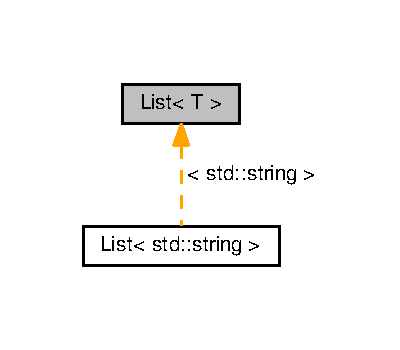
\includegraphics[width=192pt]{class_list__inherit__graph}
\end{center}
\end{figure}
\subsection*{Metody publiczne}
\begin{DoxyCompactItemize}
\item 
{\bf List} ()
\item 
{\bf $\sim$\-List} ()
\item 
int {\bf size} ()
\item 
void {\bf push\-\_\-front} (T value)
\item 
void {\bf pop\-\_\-front} ()
\item 
void {\bf push\-\_\-back} (T value)
\item 
void {\bf pop\-\_\-back} ()
\item 
void {\bf show} ()
\item 
void {\bf show\-Od\-Konca} ()
\item 
void {\bf push} (T value, int nr=0)
\item 
T \& {\bf operator[$\,$]} (int a)
\end{DoxyCompactItemize}
\subsection*{Atrybuty publiczne}
\begin{DoxyCompactItemize}
\item 
{\bf Node\-L}$<$ T $>$ $\ast$ {\bf head}
\item 
{\bf Node\-L}$<$ T $>$ $\ast$ {\bf tail}
\item 
int {\bf \-\_\-size}
\end{DoxyCompactItemize}


\subsection{Opis szczegółowy}
\subsubsection*{template$<$typename T$>$class List$<$ T $>$}



Definicja w linii 25 pliku Lista.\-hh.



\subsection{Dokumentacja konstruktora i destruktora}
\index{List@{List}!List@{List}}
\index{List@{List}!List@{List}}
\subsubsection[{List}]{\setlength{\rightskip}{0pt plus 5cm}template$<$typename T $>$ {\bf List}$<$ T $>$\-::{\bf List} (
\begin{DoxyParamCaption}
{}
\end{DoxyParamCaption}
)}\label{class_list_a5c5e27671b21b3815d4e25b953c69454}
brief Konstruktor bezparametryczny

Konstruktor bezparametryczny, ustawia parametry na 0 

Definicja w linii 101 pliku Lista.\-hh.

\index{List@{List}!$\sim$\-List@{$\sim$\-List}}
\index{$\sim$\-List@{$\sim$\-List}!List@{List}}
\subsubsection[{$\sim$\-List}]{\setlength{\rightskip}{0pt plus 5cm}template$<$typename T $>$ {\bf List}$<$ T $>$\-::$\sim${\bf List} (
\begin{DoxyParamCaption}
{}
\end{DoxyParamCaption}
)}\label{class_list_a2b58189090f6e5ce52939c9195e59e85}
brief Destruktor

Destruktor, usuwa kolejne elementy listy zaczynajac od poczatku 

Definicja w linii 112 pliku Lista.\-hh.



\subsection{Dokumentacja funkcji składowych}
\index{List@{List}!operator[$\,$]@{operator[]}}
\index{operator[$\,$]@{operator[]}!List@{List}}
\subsubsection[{operator[]}]{\setlength{\rightskip}{0pt plus 5cm}template$<$typename T$>$ T\& {\bf List}$<$ T $>$\-::operator[$\,$] (
\begin{DoxyParamCaption}
\item[{int}]{a}
\end{DoxyParamCaption}
)\hspace{0.3cm}{\ttfamily [inline]}}\label{class_list_a52f00da87e26da27b3569389ec692e83}
Przeciazony operator indeksowania zwraca referencje do elementu o indeksie a 

Definicja w linii 87 pliku Lista.\-hh.

\index{List@{List}!pop\-\_\-back@{pop\-\_\-back}}
\index{pop\-\_\-back@{pop\-\_\-back}!List@{List}}
\subsubsection[{pop\-\_\-back}]{\setlength{\rightskip}{0pt plus 5cm}template$<$typename T $>$ void {\bf List}$<$ T $>$\-::pop\-\_\-back (
\begin{DoxyParamCaption}
{}
\end{DoxyParamCaption}
)}\label{class_list_a42e1aee3e26b76b3f4d9386efa7fe8b7}
brief Funkcja zdejmuje element z konca listy

Funkcja usuwa element z konca listy \begin{DoxyPrecond}{Warunek wstępny}
Lista nie moze byc pusta 
\end{DoxyPrecond}


Definicja w linii 229 pliku Lista.\-hh.

\index{List@{List}!pop\-\_\-front@{pop\-\_\-front}}
\index{pop\-\_\-front@{pop\-\_\-front}!List@{List}}
\subsubsection[{pop\-\_\-front}]{\setlength{\rightskip}{0pt plus 5cm}template$<$typename T $>$ void {\bf List}$<$ T $>$\-::pop\-\_\-front (
\begin{DoxyParamCaption}
{}
\end{DoxyParamCaption}
)}\label{class_list_a024af4543f71544345351a45850c42d8}
brief Funkcja zdejmuje element z poczatku listy

Funkcja usuwa element z poczatku listy \begin{DoxyPrecond}{Warunek wstępny}
Lista nie moze byc pusta 
\end{DoxyPrecond}


Definicja w linii 152 pliku Lista.\-hh.

\index{List@{List}!push@{push}}
\index{push@{push}!List@{List}}
\subsubsection[{push}]{\setlength{\rightskip}{0pt plus 5cm}template$<$typename T$>$ void {\bf List}$<$ T $>$\-::push (
\begin{DoxyParamCaption}
\item[{T}]{value, }
\item[{int}]{nr = {\ttfamily 0}}
\end{DoxyParamCaption}
)}\label{class_list_a3bf27eb40044a3586f25899aa428c0c6}
brief Funkcja dodaje element przed elementem o indeksie nr

Funkcja dodaje element przed elementem o indeksie nr 
\begin{DoxyParams}[1]{Parametry}
\mbox{\tt in}  & {\em value-\/wybrany} & typ, wartosc elementu dodanego do listy \\
\hline
\mbox{\tt in}  & {\em nr-\/} & indeks elementu przed ktorym ma byc dodany element \\
\hline
\end{DoxyParams}
\begin{DoxyPrecond}{Warunek wstępny}
indeksowanie od 0 
\end{DoxyPrecond}


Definicja w linii 196 pliku Lista.\-hh.

\index{List@{List}!push\-\_\-back@{push\-\_\-back}}
\index{push\-\_\-back@{push\-\_\-back}!List@{List}}
\subsubsection[{push\-\_\-back}]{\setlength{\rightskip}{0pt plus 5cm}template$<$typename T$>$ void {\bf List}$<$ T $>$\-::push\-\_\-back (
\begin{DoxyParamCaption}
\item[{T}]{value}
\end{DoxyParamCaption}
)}\label{class_list_a6c3e359bceddd875f6d27e75de7ed15d}
brief Funkcja dodaje element na koniec listy

Funkcja dodaje element na koniec listy 
\begin{DoxyParams}[1]{Parametry}
\mbox{\tt in}  & {\em value} & -\/ typ int, wartosc elementu dodanego na koniec listy \\
\hline
\end{DoxyParams}


Definicja w linii 171 pliku Lista.\-hh.



Oto graf wywoływań tej funkcji\-:
\nopagebreak
\begin{figure}[H]
\begin{center}
\leavevmode
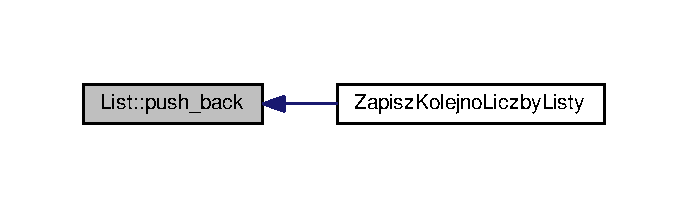
\includegraphics[width=330pt]{class_list_a6c3e359bceddd875f6d27e75de7ed15d_icgraph}
\end{center}
\end{figure}


\index{List@{List}!push\-\_\-front@{push\-\_\-front}}
\index{push\-\_\-front@{push\-\_\-front}!List@{List}}
\subsubsection[{push\-\_\-front}]{\setlength{\rightskip}{0pt plus 5cm}template$<$typename T$>$ void {\bf List}$<$ T $>$\-::push\-\_\-front (
\begin{DoxyParamCaption}
\item[{T}]{value}
\end{DoxyParamCaption}
)}\label{class_list_a2b4c57456c11a4d95bf039ae2d4e1e3c}
brief Funkcja dodaje element na poczatek listy

Funkcja sluzy do dodania elementu na poczatek listy 
\begin{DoxyParams}[1]{Parametry}
\mbox{\tt in}  & {\em value-\/typ} & int, wartosc elementu zmiennej dodanej do listy \\
\hline
\end{DoxyParams}


Definicja w linii 135 pliku Lista.\-hh.



Oto graf wywoływań tej funkcji\-:
\nopagebreak
\begin{figure}[H]
\begin{center}
\leavevmode
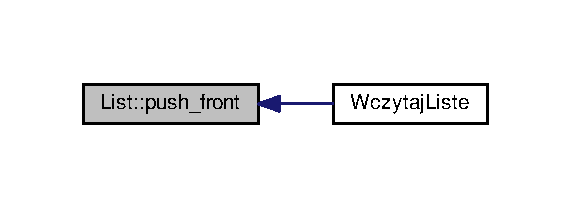
\includegraphics[width=274pt]{class_list_a2b4c57456c11a4d95bf039ae2d4e1e3c_icgraph}
\end{center}
\end{figure}


\index{List@{List}!show@{show}}
\index{show@{show}!List@{List}}
\subsubsection[{show}]{\setlength{\rightskip}{0pt plus 5cm}template$<$typename T $>$ void {\bf List}$<$ T $>$\-::show (
\begin{DoxyParamCaption}
{}
\end{DoxyParamCaption}
)}\label{class_list_aeed4e21c08aa25bf4fe12a2ac96c0f1f}
brief Funkcja wyswietla wszystkie elementy na standardowe wyjscie

brief Funkcja pokazujaca na strumieniu std\-::cout zawartosc listy

Funkcja wyswietla elementy listy 

Definicja w linii 259 pliku Lista.\-hh.

\index{List@{List}!show\-Od\-Konca@{show\-Od\-Konca}}
\index{show\-Od\-Konca@{show\-Od\-Konca}!List@{List}}
\subsubsection[{show\-Od\-Konca}]{\setlength{\rightskip}{0pt plus 5cm}template$<$typename T $>$ void {\bf List}$<$ T $>$\-::show\-Od\-Konca (
\begin{DoxyParamCaption}
{}
\end{DoxyParamCaption}
)}\label{class_list_aeecf3b2e13b4e2489c4974aacd318b33}
brief Funkcja pokazujaca na strumieniu std\-::cout zawartosc listy od konca

Funkcja wyswietla elementy listy od konca 

Definicja w linii 273 pliku Lista.\-hh.

\index{List@{List}!size@{size}}
\index{size@{size}!List@{List}}
\subsubsection[{size}]{\setlength{\rightskip}{0pt plus 5cm}template$<$typename T $>$ int {\bf List}$<$ T $>$\-::size (
\begin{DoxyParamCaption}
{}
\end{DoxyParamCaption}
)}\label{class_list_a2497bdf42246d61237aaf046c116183a}
brief Funkcja zwraca rozmiar listy

\begin{DoxyReturn}{Zwraca}
Funkcja zwraca wartosc rozmiaru listy 
\end{DoxyReturn}


Definicja w linii 125 pliku Lista.\-hh.



\subsection{Dokumentacja atrybutów składowych}
\index{List@{List}!\-\_\-size@{\-\_\-size}}
\index{\-\_\-size@{\-\_\-size}!List@{List}}
\subsubsection[{\-\_\-size}]{\setlength{\rightskip}{0pt plus 5cm}template$<$typename T$>$ int {\bf List}$<$ T $>$\-::\-\_\-size}\label{class_list_ad56fcbd2da2271dce020bb933349cba4}
brief Informacja o rozmiarze listy 

Definicja w linii 39 pliku Lista.\-hh.

\index{List@{List}!head@{head}}
\index{head@{head}!List@{List}}
\subsubsection[{head}]{\setlength{\rightskip}{0pt plus 5cm}template$<$typename T$>$ {\bf Node\-L}$<$T$>$$\ast$ {\bf List}$<$ T $>$\-::head}\label{class_list_a3caa8173609b10b902f3a578975211d6}
brief wskaznik do ktorego doczepione sa kolejne elementy listy 

Definicja w linii 31 pliku Lista.\-hh.

\index{List@{List}!tail@{tail}}
\index{tail@{tail}!List@{List}}
\subsubsection[{tail}]{\setlength{\rightskip}{0pt plus 5cm}template$<$typename T$>$ {\bf Node\-L}$<$T$>$$\ast$ {\bf List}$<$ T $>$\-::tail}\label{class_list_a40495d6470191f412dc9b51efeae43c5}
brief wskaznik pokazujacy na koniec listy 

Definicja w linii 35 pliku Lista.\-hh.



Dokumentacja dla tej klasy została wygenerowana z pliku\-:\begin{DoxyCompactItemize}
\item 
{\bf Lista.\-hh}\end{DoxyCompactItemize}

\section{Dokumentacja szablonu struktury Node$<$ T $>$}
\label{struct_node}\index{Node$<$ T $>$@{Node$<$ T $>$}}


{\ttfamily \#include $<$Kolejka.\-hh$>$}

\subsection*{Atrybuty publiczne}
\begin{DoxyCompactItemize}
\item 
T {\bf val}
\item 
{\bf Node}$<$ T $>$ $\ast$ {\bf next}
\end{DoxyCompactItemize}


\subsection{Opis szczegółowy}
\subsubsection*{template$<$typename T$>$struct Node$<$ T $>$}



Definicja w linii 10 pliku Kolejka.\-hh.



\subsection{Dokumentacja atrybutów składowych}
\index{Node@{Node}!next@{next}}
\index{next@{next}!Node@{Node}}
\subsubsection[{next}]{\setlength{\rightskip}{0pt plus 5cm}template$<$typename T$>$ {\bf Node}$<$T$>$$\ast$ {\bf Node}$<$ T $>$\-::next}\label{struct_node_a8bedac90cd0aedd2847dd49f671d4d4a}


Definicja w linii 13 pliku Kolejka.\-hh.

\index{Node@{Node}!val@{val}}
\index{val@{val}!Node@{Node}}
\subsubsection[{val}]{\setlength{\rightskip}{0pt plus 5cm}template$<$typename T$>$ T {\bf Node}$<$ T $>$\-::val}\label{struct_node_a63ca7703bf78a4ea3f6a7f32a9f705c8}


Definicja w linii 12 pliku Kolejka.\-hh.



Dokumentacja dla tej struktury została wygenerowana z pliku\-:\begin{DoxyCompactItemize}
\item 
{\bf Kolejka.\-hh}\end{DoxyCompactItemize}

\section{Node\-L$<$ T $>$ Struct Template Reference}
\label{struct_node_l}\index{Node\-L$<$ T $>$@{Node\-L$<$ T $>$}}


{\ttfamily \#include $<$Lista.\-hh$>$}

\subsection*{Public Attributes}
\begin{DoxyCompactItemize}
\item 
T {\bf val}
\item 
{\bf Node\-L}$<$ T $>$ $\ast$ {\bf next}
\end{DoxyCompactItemize}


\subsection{Detailed Description}
\subsubsection*{template$<$typename T$>$struct Node\-L$<$ T $>$}



Definition at line 11 of file Lista.\-hh.



\subsection{Member Data Documentation}
\index{Node\-L@{Node\-L}!next@{next}}
\index{next@{next}!NodeL@{Node\-L}}
\subsubsection[{next}]{\setlength{\rightskip}{0pt plus 5cm}template$<$typename T$>$ {\bf Node\-L}$<$T$>$$\ast$ {\bf Node\-L}$<$ T $>$\-::next}\label{struct_node_l_a0c3afc9e532c18b261ead8ee2218100d}


Definition at line 14 of file Lista.\-hh.

\index{Node\-L@{Node\-L}!val@{val}}
\index{val@{val}!NodeL@{Node\-L}}
\subsubsection[{val}]{\setlength{\rightskip}{0pt plus 5cm}template$<$typename T$>$ T {\bf Node\-L}$<$ T $>$\-::val}\label{struct_node_l_af8d6352b8a3b463d1a1f2dc9fa6378d6}


Definition at line 13 of file Lista.\-hh.



The documentation for this struct was generated from the following file\-:\begin{DoxyCompactItemize}
\item 
inc/{\bf Lista.\-hh}\end{DoxyCompactItemize}

\section{Dokumentacja szablonu klasy Node\-T$<$ Klucz, T $>$}
\label{class_node_t}\index{Node\-T$<$ Klucz, T $>$@{Node\-T$<$ Klucz, T $>$}}


{\ttfamily \#include $<$Node\-T.\-hh$>$}



Diagram współpracy dla Node\-T$<$ Klucz, T $>$\-:
\nopagebreak
\begin{figure}[H]
\begin{center}
\leavevmode
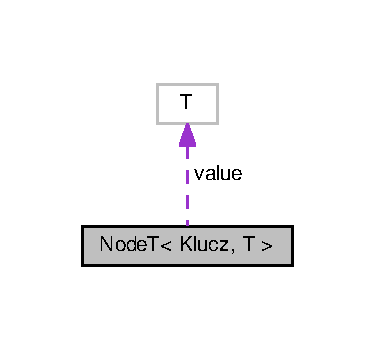
\includegraphics[width=180pt]{class_node_t__coll__graph}
\end{center}
\end{figure}
\subsection*{Metody publiczne}
\begin{DoxyCompactItemize}
\item 
{\bf Node\-T} (const Klucz \&klucz)
\item 
{\bf Node\-T} ()
\item 
Klucz \& {\bf Zwroc\-Klucz} ()
\item 
T \& {\bf Zwroc\-Value} ()
\item 
void {\bf Zmien\-Klucz} (Klucz kluczyk)
\item 
void {\bf Zmien\-Value} (T Value)
\end{DoxyCompactItemize}
\subsection*{Atrybuty prywatne}
\begin{DoxyCompactItemize}
\item 
Klucz {\bf key}
\item 
T {\bf value}
\end{DoxyCompactItemize}


\subsection{Opis szczegółowy}
\subsubsection*{template$<$typename Klucz, typename T$>$class Node\-T$<$ Klucz, T $>$}



Definicja w linii 2 pliku Node\-T.\-hh.



\subsection{Dokumentacja konstruktora i destruktora}
\index{Node\-T@{Node\-T}!Node\-T@{Node\-T}}
\index{Node\-T@{Node\-T}!NodeT@{Node\-T}}
\subsubsection[{Node\-T}]{\setlength{\rightskip}{0pt plus 5cm}template$<$typename Klucz , typename T $>$ {\bf Node\-T}$<$ Klucz, T $>$\-::{\bf Node\-T} (
\begin{DoxyParamCaption}
\item[{const Klucz \&}]{klucz}
\end{DoxyParamCaption}
)\hspace{0.3cm}{\ttfamily [inline]}}\label{class_node_t_a479bc61f1f26691f4343623f9bca812b}


Definicja w linii 8 pliku Node\-T.\-hh.

\index{Node\-T@{Node\-T}!Node\-T@{Node\-T}}
\index{Node\-T@{Node\-T}!NodeT@{Node\-T}}
\subsubsection[{Node\-T}]{\setlength{\rightskip}{0pt plus 5cm}template$<$typename Klucz , typename T $>$ {\bf Node\-T}$<$ Klucz, T $>$\-::{\bf Node\-T} (
\begin{DoxyParamCaption}
{}
\end{DoxyParamCaption}
)\hspace{0.3cm}{\ttfamily [inline]}}\label{class_node_t_ad296fb123e2e9f86b2fcd2228ed624ed}


Definicja w linii 9 pliku Node\-T.\-hh.



\subsection{Dokumentacja funkcji składowych}
\index{Node\-T@{Node\-T}!Zmien\-Klucz@{Zmien\-Klucz}}
\index{Zmien\-Klucz@{Zmien\-Klucz}!NodeT@{Node\-T}}
\subsubsection[{Zmien\-Klucz}]{\setlength{\rightskip}{0pt plus 5cm}template$<$typename Klucz , typename T $>$ void {\bf Node\-T}$<$ Klucz, T $>$\-::Zmien\-Klucz (
\begin{DoxyParamCaption}
\item[{Klucz}]{kluczyk}
\end{DoxyParamCaption}
)\hspace{0.3cm}{\ttfamily [inline]}}\label{class_node_t_ac45c9ad6860c1aeb52f2b939c5914c21}


Definicja w linii 18 pliku Node\-T.\-hh.

\index{Node\-T@{Node\-T}!Zmien\-Value@{Zmien\-Value}}
\index{Zmien\-Value@{Zmien\-Value}!NodeT@{Node\-T}}
\subsubsection[{Zmien\-Value}]{\setlength{\rightskip}{0pt plus 5cm}template$<$typename Klucz , typename T $>$ void {\bf Node\-T}$<$ Klucz, T $>$\-::Zmien\-Value (
\begin{DoxyParamCaption}
\item[{T}]{Value}
\end{DoxyParamCaption}
)\hspace{0.3cm}{\ttfamily [inline]}}\label{class_node_t_a34cc74961a82ee92dd5a55a3a40d0127}


Definicja w linii 23 pliku Node\-T.\-hh.

\index{Node\-T@{Node\-T}!Zwroc\-Klucz@{Zwroc\-Klucz}}
\index{Zwroc\-Klucz@{Zwroc\-Klucz}!NodeT@{Node\-T}}
\subsubsection[{Zwroc\-Klucz}]{\setlength{\rightskip}{0pt plus 5cm}template$<$typename Klucz , typename T $>$ Klucz\& {\bf Node\-T}$<$ Klucz, T $>$\-::Zwroc\-Klucz (
\begin{DoxyParamCaption}
{}
\end{DoxyParamCaption}
)\hspace{0.3cm}{\ttfamily [inline]}}\label{class_node_t_a0dd5663496d17b747f327cafa25e0f0d}


Definicja w linii 10 pliku Node\-T.\-hh.

\index{Node\-T@{Node\-T}!Zwroc\-Value@{Zwroc\-Value}}
\index{Zwroc\-Value@{Zwroc\-Value}!NodeT@{Node\-T}}
\subsubsection[{Zwroc\-Value}]{\setlength{\rightskip}{0pt plus 5cm}template$<$typename Klucz , typename T $>$ T\& {\bf Node\-T}$<$ Klucz, T $>$\-::Zwroc\-Value (
\begin{DoxyParamCaption}
{}
\end{DoxyParamCaption}
)\hspace{0.3cm}{\ttfamily [inline]}}\label{class_node_t_a291b8966e367bbd78f6c0d79a880ac34}


Definicja w linii 14 pliku Node\-T.\-hh.



\subsection{Dokumentacja atrybutów składowych}
\index{Node\-T@{Node\-T}!key@{key}}
\index{key@{key}!NodeT@{Node\-T}}
\subsubsection[{key}]{\setlength{\rightskip}{0pt plus 5cm}template$<$typename Klucz , typename T $>$ Klucz {\bf Node\-T}$<$ Klucz, T $>$\-::key\hspace{0.3cm}{\ttfamily [private]}}\label{class_node_t_a833d12f6ac9783f3ffd89609412aa3e5}


Definicja w linii 4 pliku Node\-T.\-hh.

\index{Node\-T@{Node\-T}!value@{value}}
\index{value@{value}!NodeT@{Node\-T}}
\subsubsection[{value}]{\setlength{\rightskip}{0pt plus 5cm}template$<$typename Klucz , typename T $>$ T {\bf Node\-T}$<$ Klucz, T $>$\-::value\hspace{0.3cm}{\ttfamily [private]}}\label{class_node_t_aedff0d9091fdfdaf53988dc427c7ded3}


Definicja w linii 5 pliku Node\-T.\-hh.



Dokumentacja dla tej klasy została wygenerowana z pliku\-:\begin{DoxyCompactItemize}
\item 
{\bf Node\-T.\-hh}\end{DoxyCompactItemize}

\section{Dokumentacja szablonu klasy Stack$<$ T $>$}
\label{class_stack}\index{Stack$<$ T $>$@{Stack$<$ T $>$}}


{\ttfamily \#include $<$Stack.\-hh$>$}

\subsection*{Metody publiczne}
\begin{DoxyCompactItemize}
\item 
{\bf Stack} (int {\bf capacity}=10)
\item 
void {\bf push} (T value)
\item 
T {\bf peek} ()
\item 
int {\bf size} ()
\item 
{\bf $\sim$\-Stack} ()
\item 
void {\bf pop} ()
\item 
T \& {\bf operator[$\,$]} (int a)
\end{DoxyCompactItemize}
\subsection*{Atrybuty publiczne}
\begin{DoxyCompactItemize}
\item 
T $\ast$ {\bf top}
\item 
int {\bf capacity}
\item 
T $\ast$ {\bf storage}
\end{DoxyCompactItemize}


\subsection{Opis szczegółowy}
\subsubsection*{template$<$typename T$>$class Stack$<$ T $>$}



Definicja w linii 11 pliku Stack.\-hh.



\subsection{Dokumentacja konstruktora i destruktora}
\index{Stack@{Stack}!Stack@{Stack}}
\index{Stack@{Stack}!Stack@{Stack}}
\subsubsection[{Stack}]{\setlength{\rightskip}{0pt plus 5cm}template$<$typename T $>$ {\bf Stack}$<$ T $>$\-::{\bf Stack} (
\begin{DoxyParamCaption}
\item[{int}]{capacity = {\ttfamily 10}}
\end{DoxyParamCaption}
)}\label{class_stack_ae6f58b476da16d508f90841455a09e5a}
Konstruktor parametryczny klasy \doxyref{Stack}{str.}{class_stack} 
\begin{DoxyParams}[1]{Parametry}
\mbox{\tt in}  & {\em capacity} & -\/ typ int, rozmiar stosu \\
\hline
\end{DoxyParams}


Definicja w linii 66 pliku Stack.\-hh.

\index{Stack@{Stack}!$\sim$\-Stack@{$\sim$\-Stack}}
\index{$\sim$\-Stack@{$\sim$\-Stack}!Stack@{Stack}}
\subsubsection[{$\sim$\-Stack}]{\setlength{\rightskip}{0pt plus 5cm}template$<$typename T $>$ {\bf Stack}$<$ T $>$\-::$\sim${\bf Stack} (
\begin{DoxyParamCaption}
{}
\end{DoxyParamCaption}
)}\label{class_stack_a9e7a00875aefbdac560ab189b7bc61d1}
Destruktor klasy \doxyref{Stack}{str.}{class_stack} 

Definicja w linii 125 pliku Stack.\-hh.



\subsection{Dokumentacja funkcji składowych}
\index{Stack@{Stack}!operator[$\,$]@{operator[]}}
\index{operator[$\,$]@{operator[]}!Stack@{Stack}}
\subsubsection[{operator[]}]{\setlength{\rightskip}{0pt plus 5cm}template$<$typename T$>$ T\& {\bf Stack}$<$ T $>$\-::operator[$\,$] (
\begin{DoxyParamCaption}
\item[{int}]{a}
\end{DoxyParamCaption}
)\hspace{0.3cm}{\ttfamily [inline]}}\label{class_stack_aa1bb812d47701510f830fa3ff36c47ad}
brief Przeciazony operator indeksowania, umozliwia traktowanie stosu jak tablicy 

Definicja w linii 54 pliku Stack.\-hh.

\index{Stack@{Stack}!peek@{peek}}
\index{peek@{peek}!Stack@{Stack}}
\subsubsection[{peek}]{\setlength{\rightskip}{0pt plus 5cm}template$<$typename T $>$ T {\bf Stack}$<$ T $>$\-::peek (
\begin{DoxyParamCaption}
{}
\end{DoxyParamCaption}
)}\label{class_stack_adcb4774ac8aa94cbc19b461da9bdee3a}
Funkcja pokazuje element znajdujacy sie na szczycie stosu \begin{DoxyPrecond}{Warunek wstępny}
Stos nie moze byc pusty 
\end{DoxyPrecond}


Definicja w linii 104 pliku Stack.\-hh.

\index{Stack@{Stack}!pop@{pop}}
\index{pop@{pop}!Stack@{Stack}}
\subsubsection[{pop}]{\setlength{\rightskip}{0pt plus 5cm}template$<$typename T $>$ void {\bf Stack}$<$ T $>$\-::pop (
\begin{DoxyParamCaption}
{}
\end{DoxyParamCaption}
)}\label{class_stack_a2723aec5c7e2611b97fcffeb7709de33}
Funkcja pop zdejmuje ostatni element ze stosu \begin{DoxyPrecond}{Warunek wstępny}
Stos nie moze byc pusty 
\end{DoxyPrecond}


Definicja w linii 136 pliku Stack.\-hh.

\index{Stack@{Stack}!push@{push}}
\index{push@{push}!Stack@{Stack}}
\subsubsection[{push}]{\setlength{\rightskip}{0pt plus 5cm}template$<$typename T $>$ void {\bf Stack}$<$ T $>$\-::push (
\begin{DoxyParamCaption}
\item[{T}]{value}
\end{DoxyParamCaption}
)}\label{class_stack_a892e33693ec391dd20c09a978b038a87}
Funkcja dodaje element na koniec tablicy stosu 
\begin{DoxyParams}[1]{Parametry}
\mbox{\tt in}  & {\em value} & -\/ typ int, wartosc dodana do stosu \\
\hline
\end{DoxyParams}
\begin{DoxyPostcond}{Warunek końcowy}
wykorzystana metoda podwajania do powiekszania stosu 
\end{DoxyPostcond}


Definicja w linii 83 pliku Stack.\-hh.



Oto graf wywoływań tej funkcji\-:
\nopagebreak
\begin{figure}[H]
\begin{center}
\leavevmode
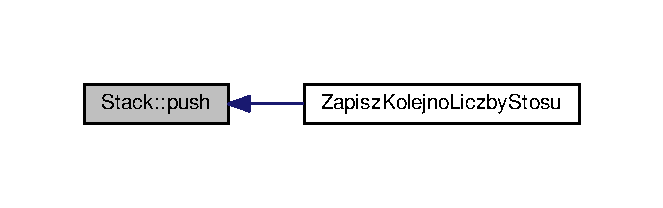
\includegraphics[width=318pt]{class_stack_a892e33693ec391dd20c09a978b038a87_icgraph}
\end{center}
\end{figure}


\index{Stack@{Stack}!size@{size}}
\index{size@{size}!Stack@{Stack}}
\subsubsection[{size}]{\setlength{\rightskip}{0pt plus 5cm}template$<$typename T $>$ int {\bf Stack}$<$ T $>$\-::size (
\begin{DoxyParamCaption}
{}
\end{DoxyParamCaption}
)}\label{class_stack_a3091d98f798b1b3e69b644d5b778c428}
Funkcja pokazuje ilosc elementow stosu \begin{DoxyReturn}{Zwraca}
zwraca ilosc elementow stosu 
\end{DoxyReturn}


Definicja w linii 116 pliku Stack.\-hh.



\subsection{Dokumentacja atrybutów składowych}
\index{Stack@{Stack}!capacity@{capacity}}
\index{capacity@{capacity}!Stack@{Stack}}
\subsubsection[{capacity}]{\setlength{\rightskip}{0pt plus 5cm}template$<$typename T$>$ int {\bf Stack}$<$ T $>$\-::capacity}\label{class_stack_a137ebd3966a796919ae064d3b205126c}


Definicja w linii 21 pliku Stack.\-hh.

\index{Stack@{Stack}!storage@{storage}}
\index{storage@{storage}!Stack@{Stack}}
\subsubsection[{storage}]{\setlength{\rightskip}{0pt plus 5cm}template$<$typename T$>$ T$\ast$ {\bf Stack}$<$ T $>$\-::storage}\label{class_stack_a93b0829d076e2a2a0fe3bf1fd0995c80}


Definicja w linii 25 pliku Stack.\-hh.

\index{Stack@{Stack}!top@{top}}
\index{top@{top}!Stack@{Stack}}
\subsubsection[{top}]{\setlength{\rightskip}{0pt plus 5cm}template$<$typename T$>$ T$\ast$ {\bf Stack}$<$ T $>$\-::top}\label{class_stack_a4ff314413cff82b4343c3094423e4345}


Definicja w linii 17 pliku Stack.\-hh.



Dokumentacja dla tej klasy została wygenerowana z pliku\-:\begin{DoxyCompactItemize}
\item 
{\bf Stack.\-hh}\end{DoxyCompactItemize}

\section{Dokumentacja klasy Tablica\-Asocjacyjna}
\label{class_tablica_asocjacyjna}\index{Tablica\-Asocjacyjna@{Tablica\-Asocjacyjna}}


{\ttfamily \#include $<$Tablica\-Asocjacyjna.\-hh$>$}



Diagram współpracy dla Tablica\-Asocjacyjna\-:
\nopagebreak
\begin{figure}[H]
\begin{center}
\leavevmode
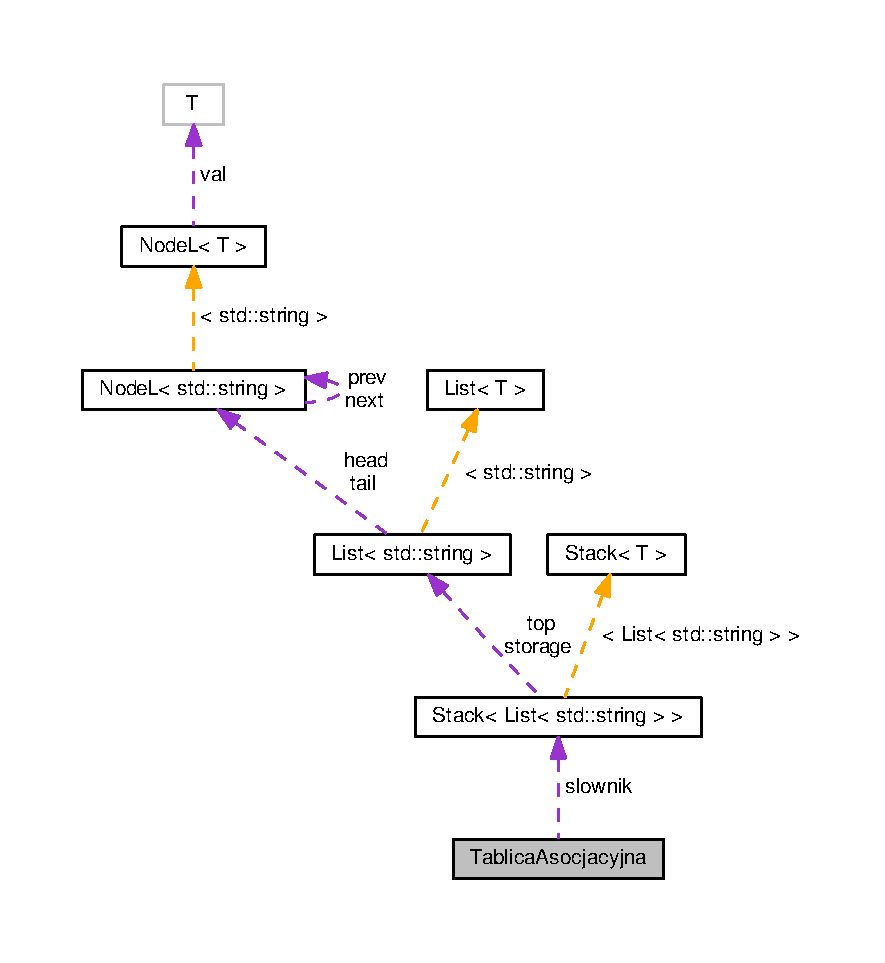
\includegraphics[width=350pt]{class_tablica_asocjacyjna__coll__graph}
\end{center}
\end{figure}
\subsection*{Metody publiczne}
\begin{DoxyCompactItemize}
\item 
{\bf Tablica\-Asocjacyjna} (unsigned long int roz)
\item 
unsigned int {\bf Haszowanie} (std\-::string nazwa)
\item 
void {\bf Wstawianie\-Do\-Tablicy} (std\-::string nazwa)
\item 
bool {\bf Wyszukaj} (std\-::string nazwa)
\item 
std\-::ostream \& {\bf Stworz\-Dane} (std\-::ostream \&Strm, unsigned int {\bf rozmiar}, int Ile\-Liter)
\item 
void {\bf Wstawianie\-Danych\-Z\-Pliku} (std\-::ifstream \&plikwe, int size)
\end{DoxyCompactItemize}
\subsection*{Atrybuty publiczne}
\begin{DoxyCompactItemize}
\item 
unsigned long int {\bf rozmiar}
\item 
unsigned int {\bf wzmocnienie}
\item 
{\bf Stack}$<$ {\bf List}$<$ std\-::string $>$ $>$ {\bf slownik}
\end{DoxyCompactItemize}


\subsection{Opis szczegółowy}


Definicja w linii 12 pliku Tablica\-Asocjacyjna.\-hh.



\subsection{Dokumentacja konstruktora i destruktora}
\index{Tablica\-Asocjacyjna@{Tablica\-Asocjacyjna}!Tablica\-Asocjacyjna@{Tablica\-Asocjacyjna}}
\index{Tablica\-Asocjacyjna@{Tablica\-Asocjacyjna}!TablicaAsocjacyjna@{Tablica\-Asocjacyjna}}
\subsubsection[{Tablica\-Asocjacyjna}]{\setlength{\rightskip}{0pt plus 5cm}Tablica\-Asocjacyjna\-::\-Tablica\-Asocjacyjna (
\begin{DoxyParamCaption}
\item[{unsigned long int}]{roz}
\end{DoxyParamCaption}
)}\label{class_tablica_asocjacyjna_aee0d297d1d45a603ff8895f029248640}
brief Konstruktor z parametrem informujacym o rozmiarze slownika

Konstruktor parametryczny klasy \doxyref{Tablica\-Asocjacyjna}{str.}{class_tablica_asocjacyjna} 
\begin{DoxyParams}{Parametry}
{\em \mbox{]}} & roz -\/ typ int, decyduje o rozmiarze slownika i wzmocnienia \\
\hline
\end{DoxyParams}


Definicja w linii 13 pliku Tablica\-Asosjacyjna.\-cpp.



\subsection{Dokumentacja funkcji składowych}
\index{Tablica\-Asocjacyjna@{Tablica\-Asocjacyjna}!Haszowanie@{Haszowanie}}
\index{Haszowanie@{Haszowanie}!TablicaAsocjacyjna@{Tablica\-Asocjacyjna}}
\subsubsection[{Haszowanie}]{\setlength{\rightskip}{0pt plus 5cm}unsigned int Tablica\-Asocjacyjna\-::\-Haszowanie (
\begin{DoxyParamCaption}
\item[{std\-::string}]{nazwa}
\end{DoxyParamCaption}
)}\label{class_tablica_asocjacyjna_a2308399ff078591ba1ba87a74a3d8031}
brief Funkcja haszujaca dany string

Funkcja haszujaca dany string 
\begin{DoxyParams}{Parametry}
{\em \mbox{]}} & nazwa -\/ string z ktorego zostanie obliczona wartosc hasz \\
\hline
\end{DoxyParams}
\begin{DoxyReturn}{Zwraca}
unsigned int-\/ wartosc haszu z podanego stringu 
\end{DoxyReturn}


Definicja w linii 50 pliku Tablica\-Asosjacyjna.\-cpp.



Oto graf wywoływań tej funkcji\-:
\nopagebreak
\begin{figure}[H]
\begin{center}
\leavevmode
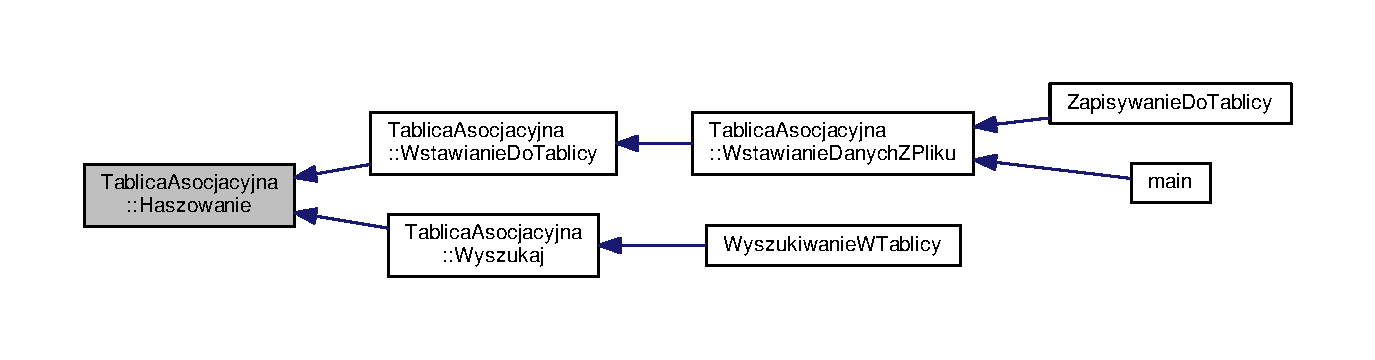
\includegraphics[width=350pt]{class_tablica_asocjacyjna_a2308399ff078591ba1ba87a74a3d8031_icgraph}
\end{center}
\end{figure}


\index{Tablica\-Asocjacyjna@{Tablica\-Asocjacyjna}!Stworz\-Dane@{Stworz\-Dane}}
\index{Stworz\-Dane@{Stworz\-Dane}!TablicaAsocjacyjna@{Tablica\-Asocjacyjna}}
\subsubsection[{Stworz\-Dane}]{\setlength{\rightskip}{0pt plus 5cm}ostream \& Tablica\-Asocjacyjna\-::\-Stworz\-Dane (
\begin{DoxyParamCaption}
\item[{std\-::ostream \&}]{Strm, }
\item[{unsigned int}]{rozmiar, }
\item[{int}]{Ile\-Liter}
\end{DoxyParamCaption}
)}\label{class_tablica_asocjacyjna_a4362e8b064c99c6c7129b71ceb76c4c4}
brief Funkcja tworzaca przykladowy zestaw danych stringow

Funkcja tworzaca przykladowy zestaw danych stringow 
\begin{DoxyParams}{Parametry}
{\em \mbox{]}} & Strm -\/ referencja do strumieinia wyjsciowego \\
\hline
{\em \mbox{]}} & rozmiarek -\/ typ u\-\_\-int , ilosc stworzonych stringow \\
\hline
{\em \mbox{]}} & Ile\-Liter -\/ typ int, jak wiele liter ma posiadac dany string \\
\hline
\end{DoxyParams}


Definicja w linii 86 pliku Tablica\-Asosjacyjna.\-cpp.

\index{Tablica\-Asocjacyjna@{Tablica\-Asocjacyjna}!Wstawianie\-Danych\-Z\-Pliku@{Wstawianie\-Danych\-Z\-Pliku}}
\index{Wstawianie\-Danych\-Z\-Pliku@{Wstawianie\-Danych\-Z\-Pliku}!TablicaAsocjacyjna@{Tablica\-Asocjacyjna}}
\subsubsection[{Wstawianie\-Danych\-Z\-Pliku}]{\setlength{\rightskip}{0pt plus 5cm}void Tablica\-Asocjacyjna\-::\-Wstawianie\-Danych\-Z\-Pliku (
\begin{DoxyParamCaption}
\item[{std\-::ifstream \&}]{plikwe, }
\item[{int}]{size}
\end{DoxyParamCaption}
)}\label{class_tablica_asocjacyjna_ab5c01397c7d79785c794e418753697f5}
brief Funkcja wstawia dane z pliku do slownika z wykorzystaniem haszowania

Funkcja wstawia dane z pliku do slownika z wykorzystaniem haszowania 
\begin{DoxyParams}{Parametry}
{\em \mbox{]}} & plikwe -\/ referencja do strumienia wejsciowego \\
\hline
{\em \mbox{]}} & size -\/ typ int, ilosc liczb wczytanych z pliku do slownika \\
\hline
\end{DoxyParams}


Definicja w linii 36 pliku Tablica\-Asosjacyjna.\-cpp.



Oto graf wywołań dla tej funkcji\-:
\nopagebreak
\begin{figure}[H]
\begin{center}
\leavevmode
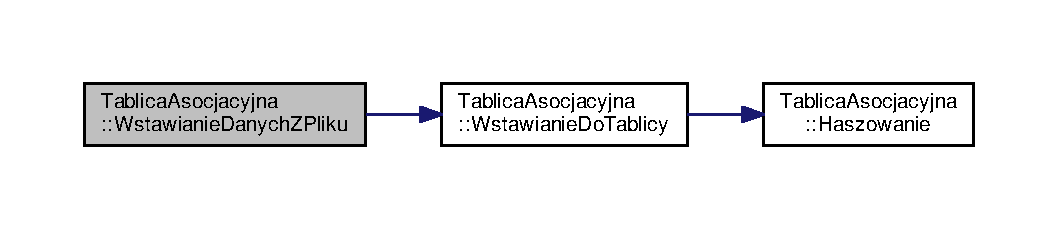
\includegraphics[width=350pt]{class_tablica_asocjacyjna_ab5c01397c7d79785c794e418753697f5_cgraph}
\end{center}
\end{figure}




Oto graf wywoływań tej funkcji\-:
\nopagebreak
\begin{figure}[H]
\begin{center}
\leavevmode
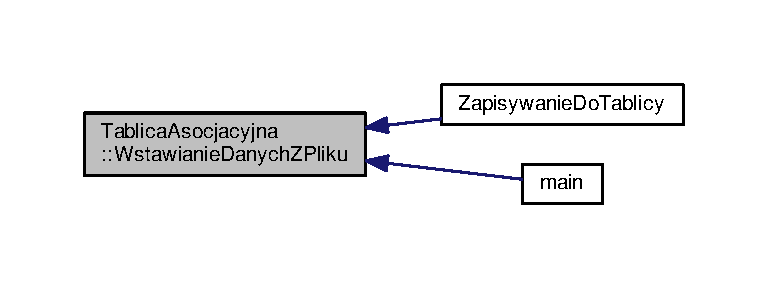
\includegraphics[width=350pt]{class_tablica_asocjacyjna_ab5c01397c7d79785c794e418753697f5_icgraph}
\end{center}
\end{figure}


\index{Tablica\-Asocjacyjna@{Tablica\-Asocjacyjna}!Wstawianie\-Do\-Tablicy@{Wstawianie\-Do\-Tablicy}}
\index{Wstawianie\-Do\-Tablicy@{Wstawianie\-Do\-Tablicy}!TablicaAsocjacyjna@{Tablica\-Asocjacyjna}}
\subsubsection[{Wstawianie\-Do\-Tablicy}]{\setlength{\rightskip}{0pt plus 5cm}void Tablica\-Asocjacyjna\-::\-Wstawianie\-Do\-Tablicy (
\begin{DoxyParamCaption}
\item[{std\-::string}]{nazwa}
\end{DoxyParamCaption}
)}\label{class_tablica_asocjacyjna_a74a7c9eb56a52c12f5048c9348771cc4}
brief Funkcja Wstawiajaca do slownika dany string, wykorzystujaca haszowanie

Funkcja wyszukujaca dany string w slowniku z wykorzystaniem haszowania 
\begin{DoxyParams}{Parametry}
{\em \mbox{]}} & nazwa -\/ nazwa stringu, ktory bedzie haszowany i umieszczony w slowniku \\
\hline
\end{DoxyParams}


Definicja w linii 25 pliku Tablica\-Asosjacyjna.\-cpp.



Oto graf wywołań dla tej funkcji\-:
\nopagebreak
\begin{figure}[H]
\begin{center}
\leavevmode
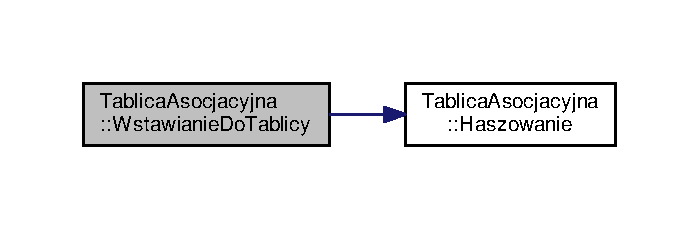
\includegraphics[width=336pt]{class_tablica_asocjacyjna_a74a7c9eb56a52c12f5048c9348771cc4_cgraph}
\end{center}
\end{figure}




Oto graf wywoływań tej funkcji\-:
\nopagebreak
\begin{figure}[H]
\begin{center}
\leavevmode
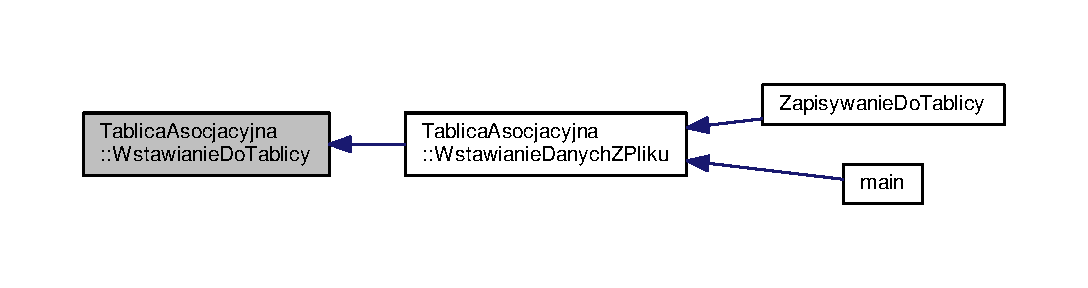
\includegraphics[width=350pt]{class_tablica_asocjacyjna_a74a7c9eb56a52c12f5048c9348771cc4_icgraph}
\end{center}
\end{figure}


\index{Tablica\-Asocjacyjna@{Tablica\-Asocjacyjna}!Wyszukaj@{Wyszukaj}}
\index{Wyszukaj@{Wyszukaj}!TablicaAsocjacyjna@{Tablica\-Asocjacyjna}}
\subsubsection[{Wyszukaj}]{\setlength{\rightskip}{0pt plus 5cm}bool Tablica\-Asocjacyjna\-::\-Wyszukaj (
\begin{DoxyParamCaption}
\item[{std\-::string}]{nazwa}
\end{DoxyParamCaption}
)}\label{class_tablica_asocjacyjna_a21de0956122e8dbf35bdc87951544210}
brief Funkcja wyszukujaca dany string w slowniku z wykorzystaniem haszowania

Funkcja wyszukujaca dany string w slowniku z wykorzystaniem haszowania 
\begin{DoxyParams}{Parametry}
{\em \mbox{]}} & nazwa -\/ string z ktorego zostanie obliczona wartosc hasz \\
\hline
\end{DoxyParams}
\begin{DoxyReturn}{Zwraca}
true-\/jesli dany string znaleziono, false -\/ nie znaleziono 
\end{DoxyReturn}


Definicja w linii 64 pliku Tablica\-Asosjacyjna.\-cpp.



Oto graf wywołań dla tej funkcji\-:
\nopagebreak
\begin{figure}[H]
\begin{center}
\leavevmode
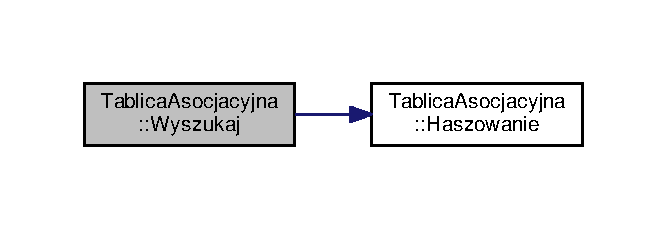
\includegraphics[width=320pt]{class_tablica_asocjacyjna_a21de0956122e8dbf35bdc87951544210_cgraph}
\end{center}
\end{figure}




Oto graf wywoływań tej funkcji\-:
\nopagebreak
\begin{figure}[H]
\begin{center}
\leavevmode
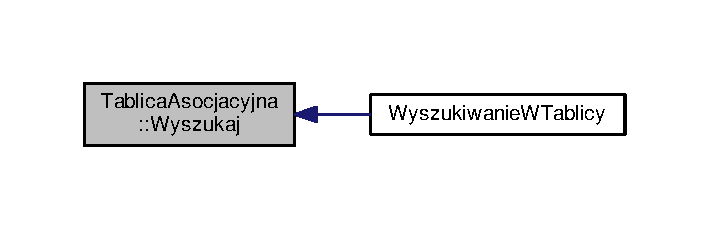
\includegraphics[width=340pt]{class_tablica_asocjacyjna_a21de0956122e8dbf35bdc87951544210_icgraph}
\end{center}
\end{figure}




\subsection{Dokumentacja atrybutów składowych}
\index{Tablica\-Asocjacyjna@{Tablica\-Asocjacyjna}!rozmiar@{rozmiar}}
\index{rozmiar@{rozmiar}!TablicaAsocjacyjna@{Tablica\-Asocjacyjna}}
\subsubsection[{rozmiar}]{\setlength{\rightskip}{0pt plus 5cm}unsigned long int Tablica\-Asocjacyjna\-::rozmiar}\label{class_tablica_asocjacyjna_a65be6187d9e5b32f0350662529bee6e3}
brief Informacja o ilosci elementow w slowniku 

Definicja w linii 19 pliku Tablica\-Asocjacyjna.\-hh.

\index{Tablica\-Asocjacyjna@{Tablica\-Asocjacyjna}!slownik@{slownik}}
\index{slownik@{slownik}!TablicaAsocjacyjna@{Tablica\-Asocjacyjna}}
\subsubsection[{slownik}]{\setlength{\rightskip}{0pt plus 5cm}{\bf Stack}$<${\bf List}$<$std\-::string$>$ $>$ Tablica\-Asocjacyjna\-::slownik}\label{class_tablica_asocjacyjna_adaacea4af5471d9977e082bb1b4c58f2}
brief Zmienna przechowujaca dane wlasciwe(stringi) 

Definicja w linii 27 pliku Tablica\-Asocjacyjna.\-hh.

\index{Tablica\-Asocjacyjna@{Tablica\-Asocjacyjna}!wzmocnienie@{wzmocnienie}}
\index{wzmocnienie@{wzmocnienie}!TablicaAsocjacyjna@{Tablica\-Asocjacyjna}}
\subsubsection[{wzmocnienie}]{\setlength{\rightskip}{0pt plus 5cm}unsigned int Tablica\-Asocjacyjna\-::wzmocnienie}\label{class_tablica_asocjacyjna_af9e8cf03f24acda77d70c27b0fef0b1c}
brief Zmienna wymagana do haszowania 

Definicja w linii 23 pliku Tablica\-Asocjacyjna.\-hh.



Dokumentacja dla tej klasy została wygenerowana z plików\-:\begin{DoxyCompactItemize}
\item 
{\bf Tablica\-Asocjacyjna.\-hh}\item 
{\bf Tablica\-Asosjacyjna.\-cpp}\end{DoxyCompactItemize}

\chapter{Dokumentacja plików}
\section{Dokumentacja pliku Benchmark.\-hh}
\label{_benchmark_8hh}\index{Benchmark.\-hh@{Benchmark.\-hh}}


Klasa \doxyref{Benchmark}{str.}{class_benchmark} sluzy do przechowywania wynikow zlozonosci obliczeniowej i danych wejsciowych,generowania liczb rozkladu Gaussowego.  


{\ttfamily \#include $<$iostream$>$}\\*
{\ttfamily \#include $<$chrono$>$}\\*
{\ttfamily \#include $<$cstdlib$>$}\\*
{\ttfamily \#include $<$ctime$>$}\\*
{\ttfamily \#include $<$cmath$>$}\\*
{\ttfamily \#include $<$fstream$>$}\\*
Wykres zależności załączania dla Benchmark.\-hh\-:
\nopagebreak
\begin{figure}[H]
\begin{center}
\leavevmode
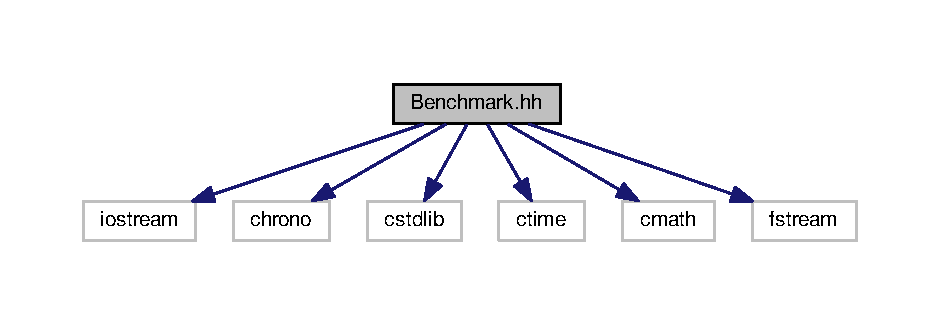
\includegraphics[width=350pt]{_benchmark_8hh__incl}
\end{center}
\end{figure}
Ten wykres pokazuje, które pliki bezpośrednio lub pośrednio załączają ten plik\-:
\nopagebreak
\begin{figure}[H]
\begin{center}
\leavevmode
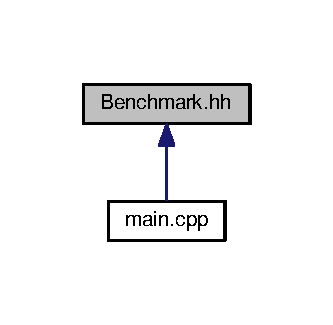
\includegraphics[width=216pt]{_benchmark_8hh__dep__incl}
\end{center}
\end{figure}
\subsection*{Komponenty}
\begin{DoxyCompactItemize}
\item 
class {\bf Benchmark$<$ T $>$}
\end{DoxyCompactItemize}
\subsection*{Funkcje}
\begin{DoxyCompactItemize}
\item 
{\footnotesize template$<$typename T $>$ }\\std\-::ostream \& {\bf operator$<$$<$} (std\-::ostream \&Strm, const {\bf Benchmark}$<$ T $>$ \&ben)
\item 
{\footnotesize template$<$typename T $>$ }\\std\-::istream \& {\bf operator$>$$>$} (std\-::istream \&Strm, {\bf Benchmark}$<$ T $>$ \&ben)
\end{DoxyCompactItemize}


\subsection{Dokumentacja funkcji}
\index{Benchmark.\-hh@{Benchmark.\-hh}!operator$<$$<$@{operator$<$$<$}}
\index{operator$<$$<$@{operator$<$$<$}!Benchmark.hh@{Benchmark.\-hh}}
\subsubsection[{operator$<$$<$}]{\setlength{\rightskip}{0pt plus 5cm}template$<$typename T $>$ std\-::ostream\& operator$<$$<$ (
\begin{DoxyParamCaption}
\item[{std\-::ostream \&}]{Strm, }
\item[{const {\bf Benchmark}$<$ T $>$ \&}]{ben}
\end{DoxyParamCaption}
)}\label{_benchmark_8hh_a09165957505edd311379cffe3322da36}
Funkcja operatorowa pozwala na wypisanie wszystkich liczb tablicy Liczby\-Gaussowe 
\begin{DoxyParams}[1]{Parametry}
\mbox{\tt in,out}  & {\em \&\-Strm} & -\/ referencja do strumienia wyjsciowego \\
\hline
\mbox{\tt in,out}  & {\em \&ben} & refencja do klasy typu \doxyref{Benchmark}{str.}{class_benchmark} \\
\hline
\end{DoxyParams}
\begin{DoxyReturn}{Zwraca}
Zwraca referencje do strumienia wyjsciowego 
\end{DoxyReturn}
\begin{DoxyPrecond}{Warunek wstępny}
Poprawne wczytanie liczb tablicy Liczby\-Gaussowe 
\end{DoxyPrecond}


Definicja w linii 140 pliku Benchmark.\-hh.

\index{Benchmark.\-hh@{Benchmark.\-hh}!operator$>$$>$@{operator$>$$>$}}
\index{operator$>$$>$@{operator$>$$>$}!Benchmark.hh@{Benchmark.\-hh}}
\subsubsection[{operator$>$$>$}]{\setlength{\rightskip}{0pt plus 5cm}template$<$typename T $>$ std\-::istream\& operator$>$$>$ (
\begin{DoxyParamCaption}
\item[{std\-::istream \&}]{Strm, }
\item[{{\bf Benchmark}$<$ T $>$ \&}]{ben}
\end{DoxyParamCaption}
)}\label{_benchmark_8hh_a849f5a7f6bcdc2c75a3d6bc6367f792e}
Funkcja operatorowa pozwala na wczytanie liczby typu double do tablicy Liczby\-Gaussowe 
\begin{DoxyParams}[1]{Parametry}
\mbox{\tt in,out}  & {\em \&\-Strm} & -\/ referencja do strumienia wejsciowego \\
\hline
\mbox{\tt in,out}  & {\em \&ben} & referencja do klasy typu \doxyref{Benchmark}{str.}{class_benchmark} \\
\hline
\end{DoxyParams}
\begin{DoxyReturn}{Zwraca}
Zwraca referencje do strumienia wejsciowego 
\end{DoxyReturn}
\begin{DoxyPrecond}{Warunek wstępny}
Liczba tylko typu double 
\end{DoxyPrecond}


Definicja w linii 158 pliku Benchmark.\-hh.


\section{Dokumentacja pliku Hasz\-Wyszukaj.\-cpp}
\label{_hasz_wyszukaj_8cpp}\index{Hasz\-Wyszukaj.\-cpp@{Hasz\-Wyszukaj.\-cpp}}
{\ttfamily \#include $<$fstream$>$}\\*
{\ttfamily \#include $<$string$>$}\\*
{\ttfamily \#include \char`\"{}Hasz\-Wyszukaj.\-hh\char`\"{}}\\*
Wykres zależności załączania dla Hasz\-Wyszukaj.\-cpp\-:
\nopagebreak
\begin{figure}[H]
\begin{center}
\leavevmode
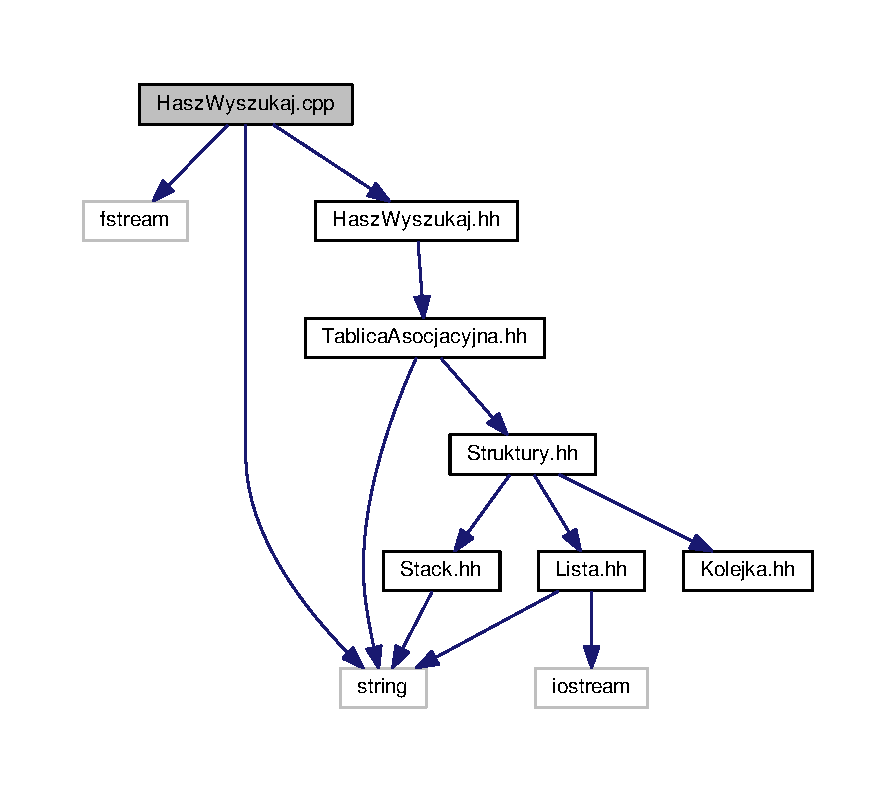
\includegraphics[width=350pt]{_hasz_wyszukaj_8cpp__incl}
\end{center}
\end{figure}
\subsection*{Funkcje}
\begin{DoxyCompactItemize}
\item 
void {\bf Zapisywanie\-Do\-Tablicy} ({\bf Tablica\-Asocjacyjna} $\ast$a, int rozmiar)
\item 
void {\bf Wyszukiwanie\-W\-Tablicy} ({\bf Tablica\-Asocjacyjna} $\ast$a, int rozmiar)
\end{DoxyCompactItemize}


\subsection{Dokumentacja funkcji}
\index{Hasz\-Wyszukaj.\-cpp@{Hasz\-Wyszukaj.\-cpp}!Wyszukiwanie\-W\-Tablicy@{Wyszukiwanie\-W\-Tablicy}}
\index{Wyszukiwanie\-W\-Tablicy@{Wyszukiwanie\-W\-Tablicy}!HaszWyszukaj.cpp@{Hasz\-Wyszukaj.\-cpp}}
\subsubsection[{Wyszukiwanie\-W\-Tablicy}]{\setlength{\rightskip}{0pt plus 5cm}void Wyszukiwanie\-W\-Tablicy (
\begin{DoxyParamCaption}
\item[{{\bf Tablica\-Asocjacyjna} $\ast$}]{a, }
\item[{int}]{rozmiar}
\end{DoxyParamCaption}
)}\label{_hasz_wyszukaj_8cpp_a9992228371d23ae098e1050ac5bd85ef}
Funkcja sluzy do odnajdowania elementow w tablicy haszowanej. 
\begin{DoxyParams}{Parametry}
{\em \mbox{]}} & a -\/ wskaznik na klase \doxyref{Tablica\-Asocjacyjna}{str.}{class_tablica_asocjacyjna} \\
\hline
{\em \mbox{]}} & rozmiar -\/ jak wiele elementow ma byc wyszukanych \\
\hline
\end{DoxyParams}


Definicja w linii 24 pliku Hasz\-Wyszukaj.\-cpp.



Oto graf wywołań dla tej funkcji\-:
\nopagebreak
\begin{figure}[H]
\begin{center}
\leavevmode
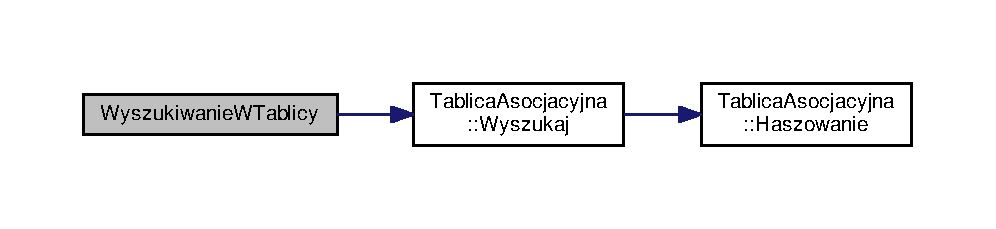
\includegraphics[width=350pt]{_hasz_wyszukaj_8cpp_a9992228371d23ae098e1050ac5bd85ef_cgraph}
\end{center}
\end{figure}


\index{Hasz\-Wyszukaj.\-cpp@{Hasz\-Wyszukaj.\-cpp}!Zapisywanie\-Do\-Tablicy@{Zapisywanie\-Do\-Tablicy}}
\index{Zapisywanie\-Do\-Tablicy@{Zapisywanie\-Do\-Tablicy}!HaszWyszukaj.cpp@{Hasz\-Wyszukaj.\-cpp}}
\subsubsection[{Zapisywanie\-Do\-Tablicy}]{\setlength{\rightskip}{0pt plus 5cm}void Zapisywanie\-Do\-Tablicy (
\begin{DoxyParamCaption}
\item[{{\bf Tablica\-Asocjacyjna} $\ast$}]{a, }
\item[{int}]{rozmiar}
\end{DoxyParamCaption}
)}\label{_hasz_wyszukaj_8cpp_a907031016d0a93a0a4e58ca717dafce0}
Funkcja sluzy do zapisywania do tablicy z wykorzystaniem haszowania. 
\begin{DoxyParams}{Parametry}
{\em \mbox{]}} & a -\/ wskaznik na klase \doxyref{Tablica\-Asocjacyjna}{str.}{class_tablica_asocjacyjna} \\
\hline
{\em \mbox{]}} & rozmiar -\/ jak wiele elementow ma byc wstawionych \\
\hline
\end{DoxyParams}


Definicja w linii 12 pliku Hasz\-Wyszukaj.\-cpp.



Oto graf wywołań dla tej funkcji\-:
\nopagebreak
\begin{figure}[H]
\begin{center}
\leavevmode
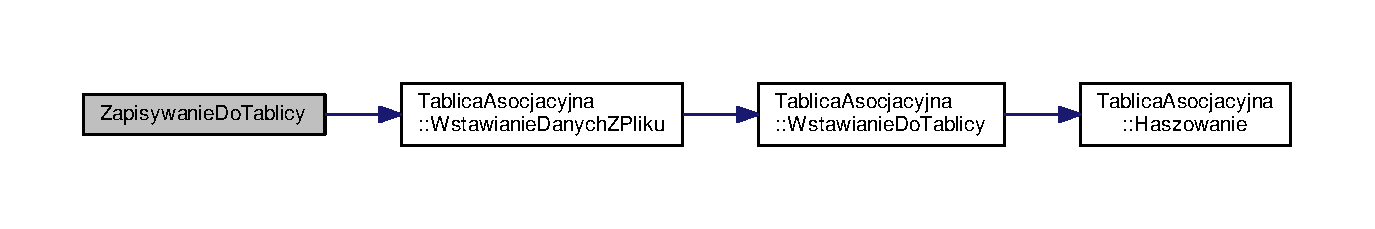
\includegraphics[width=350pt]{_hasz_wyszukaj_8cpp_a907031016d0a93a0a4e58ca717dafce0_cgraph}
\end{center}
\end{figure}



\section{Dokumentacja pliku Hasz\-Wyszukaj.\-hh}
\label{_hasz_wyszukaj_8hh}\index{Hasz\-Wyszukaj.\-hh@{Hasz\-Wyszukaj.\-hh}}
{\ttfamily \#include \char`\"{}Tablica\-Asocjacyjna.\-hh\char`\"{}}\\*
Wykres zależności załączania dla Hasz\-Wyszukaj.\-hh\-:
\nopagebreak
\begin{figure}[H]
\begin{center}
\leavevmode
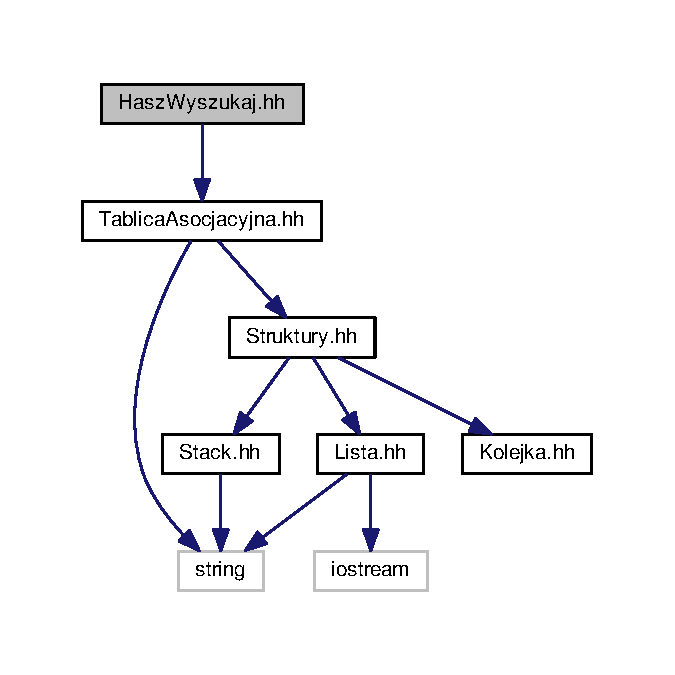
\includegraphics[width=324pt]{_hasz_wyszukaj_8hh__incl}
\end{center}
\end{figure}
Ten wykres pokazuje, które pliki bezpośrednio lub pośrednio załączają ten plik\-:
\nopagebreak
\begin{figure}[H]
\begin{center}
\leavevmode
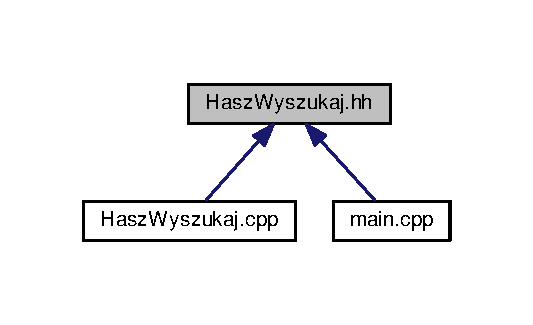
\includegraphics[width=256pt]{_hasz_wyszukaj_8hh__dep__incl}
\end{center}
\end{figure}
\subsection*{Funkcje}
\begin{DoxyCompactItemize}
\item 
void {\bf Zapisywanie\-Do\-Tablicy} ({\bf Tablica\-Asocjacyjna} $\ast$a, int rozmiar)
\item 
void {\bf Wyszukiwanie\-W\-Tablicy} ({\bf Tablica\-Asocjacyjna} $\ast$a, int rozmiar)
\end{DoxyCompactItemize}


\subsection{Dokumentacja funkcji}
\index{Hasz\-Wyszukaj.\-hh@{Hasz\-Wyszukaj.\-hh}!Wyszukiwanie\-W\-Tablicy@{Wyszukiwanie\-W\-Tablicy}}
\index{Wyszukiwanie\-W\-Tablicy@{Wyszukiwanie\-W\-Tablicy}!HaszWyszukaj.hh@{Hasz\-Wyszukaj.\-hh}}
\subsubsection[{Wyszukiwanie\-W\-Tablicy}]{\setlength{\rightskip}{0pt plus 5cm}void Wyszukiwanie\-W\-Tablicy (
\begin{DoxyParamCaption}
\item[{{\bf Tablica\-Asocjacyjna} $\ast$}]{a, }
\item[{int}]{rozmiar}
\end{DoxyParamCaption}
)}\label{_hasz_wyszukaj_8hh_a9992228371d23ae098e1050ac5bd85ef}
brief Funkcja sluzy do odnajdowania elementow w tablicy haszowanej.

Funkcja sluzy do odnajdowania elementow w tablicy haszowanej. 
\begin{DoxyParams}{Parametry}
{\em \mbox{]}} & a -\/ wskaznik na klase \doxyref{Tablica\-Asocjacyjna}{str.}{class_tablica_asocjacyjna} \\
\hline
{\em \mbox{]}} & rozmiar -\/ jak wiele elementow ma byc wyszukanych \\
\hline
\end{DoxyParams}


Definicja w linii 24 pliku Hasz\-Wyszukaj.\-cpp.



Oto graf wywołań dla tej funkcji\-:
\nopagebreak
\begin{figure}[H]
\begin{center}
\leavevmode
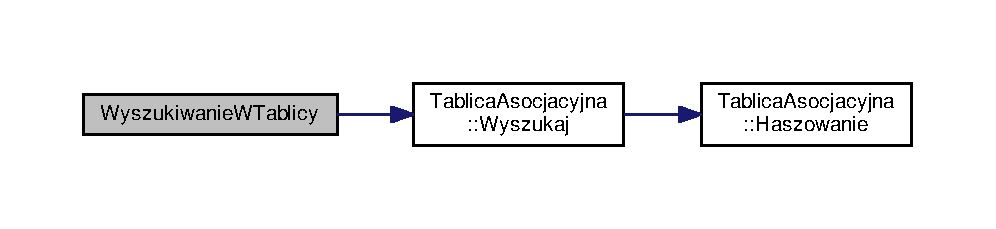
\includegraphics[width=350pt]{_hasz_wyszukaj_8hh_a9992228371d23ae098e1050ac5bd85ef_cgraph}
\end{center}
\end{figure}


\index{Hasz\-Wyszukaj.\-hh@{Hasz\-Wyszukaj.\-hh}!Zapisywanie\-Do\-Tablicy@{Zapisywanie\-Do\-Tablicy}}
\index{Zapisywanie\-Do\-Tablicy@{Zapisywanie\-Do\-Tablicy}!HaszWyszukaj.hh@{Hasz\-Wyszukaj.\-hh}}
\subsubsection[{Zapisywanie\-Do\-Tablicy}]{\setlength{\rightskip}{0pt plus 5cm}void Zapisywanie\-Do\-Tablicy (
\begin{DoxyParamCaption}
\item[{{\bf Tablica\-Asocjacyjna} $\ast$}]{a, }
\item[{int}]{rozmiar}
\end{DoxyParamCaption}
)}\label{_hasz_wyszukaj_8hh_a907031016d0a93a0a4e58ca717dafce0}
brief Funkcja sluzy do zapisywania do tablicy z wykorzystaniem haszowania.

Funkcja sluzy do zapisywania do tablicy z wykorzystaniem haszowania. 
\begin{DoxyParams}{Parametry}
{\em \mbox{]}} & a -\/ wskaznik na klase \doxyref{Tablica\-Asocjacyjna}{str.}{class_tablica_asocjacyjna} \\
\hline
{\em \mbox{]}} & rozmiar -\/ jak wiele elementow ma byc wstawionych \\
\hline
\end{DoxyParams}


Definicja w linii 12 pliku Hasz\-Wyszukaj.\-cpp.



Oto graf wywołań dla tej funkcji\-:
\nopagebreak
\begin{figure}[H]
\begin{center}
\leavevmode
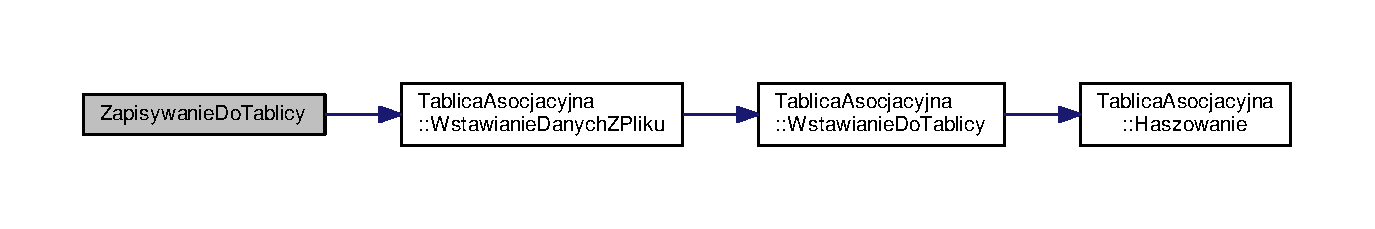
\includegraphics[width=350pt]{_hasz_wyszukaj_8hh_a907031016d0a93a0a4e58ca717dafce0_cgraph}
\end{center}
\end{figure}



\section{Dokumentacja pliku Kolejka.\-hh}
\label{_kolejka_8hh}\index{Kolejka.\-hh@{Kolejka.\-hh}}


Struktura przechowujaca wartosc wezla i wskaznik na nastepny element typu \doxyref{Node}{str.}{struct_node}.  


Ten wykres pokazuje, które pliki bezpośrednio lub pośrednio załączają ten plik\-:\nopagebreak
\begin{figure}[H]
\begin{center}
\leavevmode
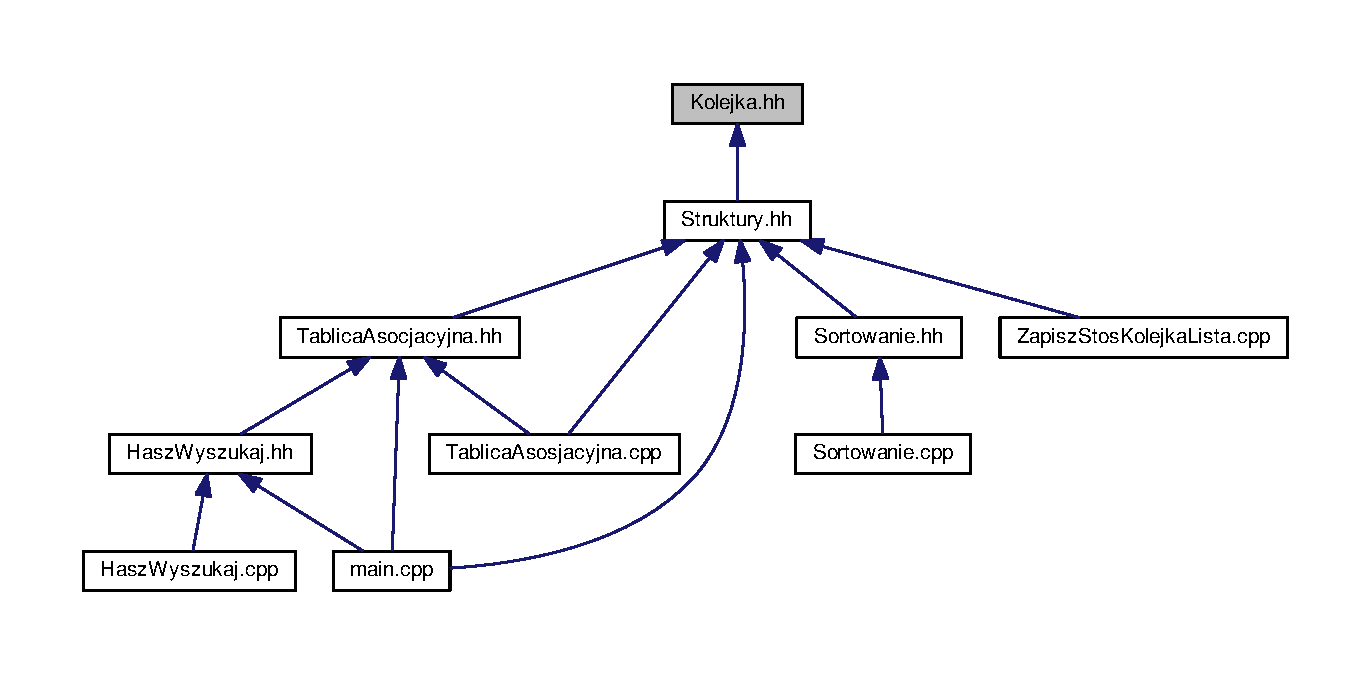
\includegraphics[width=218pt]{_kolejka_8hh__dep__incl}
\end{center}
\end{figure}
\subsection*{Komponenty}
\begin{DoxyCompactItemize}
\item 
struct {\bf Node$<$ T $>$}
\item 
class {\bf Kolejka$<$ T $>$}
\begin{DoxyCompactList}\small\item\em klasa \doxyref{Kolejka}{str.}{class_kolejka} sluzy do wykonywania podstawowych operacji na Kolejce\-: dodaj,odejmij element. Przechowuje informacje o ilosci wszysktich elementow. \end{DoxyCompactList}\end{DoxyCompactItemize}

\section{inc/\-Lista.hh File Reference}
\label{_lista_8hh}\index{inc/\-Lista.\-hh@{inc/\-Lista.\-hh}}


Struktura przechowujaca wartosc wezla i wskaznik na nastepny element typu \doxyref{Node}{p.}{struct_node}.  


This graph shows which files directly or indirectly include this file\-:\nopagebreak
\begin{figure}[H]
\begin{center}
\leavevmode
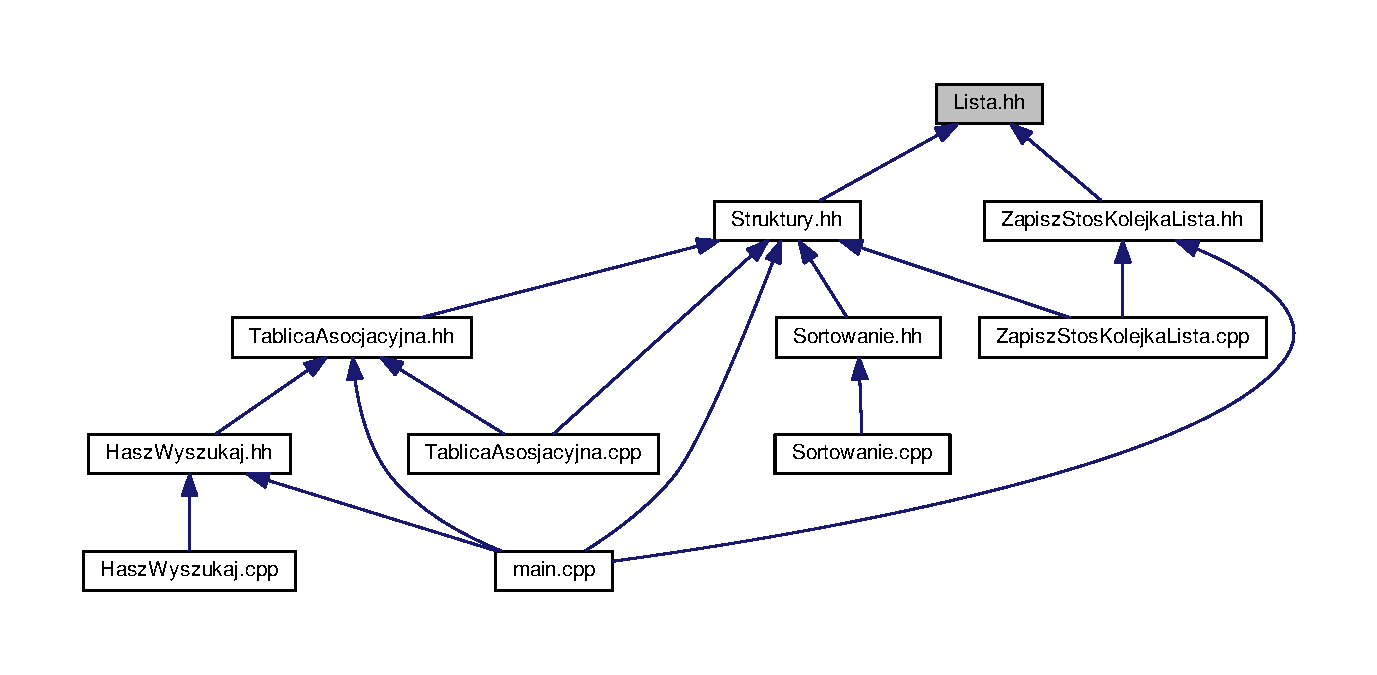
\includegraphics[width=152pt]{_lista_8hh__dep__incl}
\end{center}
\end{figure}
\subsection*{Classes}
\begin{DoxyCompactItemize}
\item 
struct {\bf Node\-L$<$ T $>$}
\item 
class {\bf List$<$ T $>$}
\begin{DoxyCompactList}\small\item\em klasa \doxyref{List}{p.}{class_list} sluzy do wykonywania podstawowych operacji na Liscie\-: dodaj,odejmij element. Przechowuje informacje o ilosci wszysktich elementow. \end{DoxyCompactList}\end{DoxyCompactItemize}


\subsection{Detailed Description}
Struktura przechowujaca wartosc wezla i wskaznik na nastepny element typu \doxyref{Node}{p.}{struct_node}. 

Definition in file {\bf Lista.\-hh}.


\section{Dokumentacja pliku main.\-cpp}
\label{main_8cpp}\index{main.\-cpp@{main.\-cpp}}
{\ttfamily \#include $<$iostream$>$}\\*
{\ttfamily \#include $<$fstream$>$}\\*
{\ttfamily \#include $<$string$>$}\\*
{\ttfamily \#include $<$cstdlib$>$}\\*
{\ttfamily \#include \char`\"{}Benchmark.\-hh\char`\"{}}\\*
{\ttfamily \#include \char`\"{}Zapisz\-Stos\-Kolejka\-Lista.\-hh\char`\"{}}\\*
{\ttfamily \#include \char`\"{}Operacje\-Na\-Plikach.\-hh\char`\"{}}\\*
{\ttfamily \#include \char`\"{}Struktury.\-hh\char`\"{}}\\*
{\ttfamily \#include \char`\"{}Sortowanie.\-hh\char`\"{}}\\*
Wykres zależności załączania dla main.\-cpp\-:
\nopagebreak
\begin{figure}[H]
\begin{center}
\leavevmode
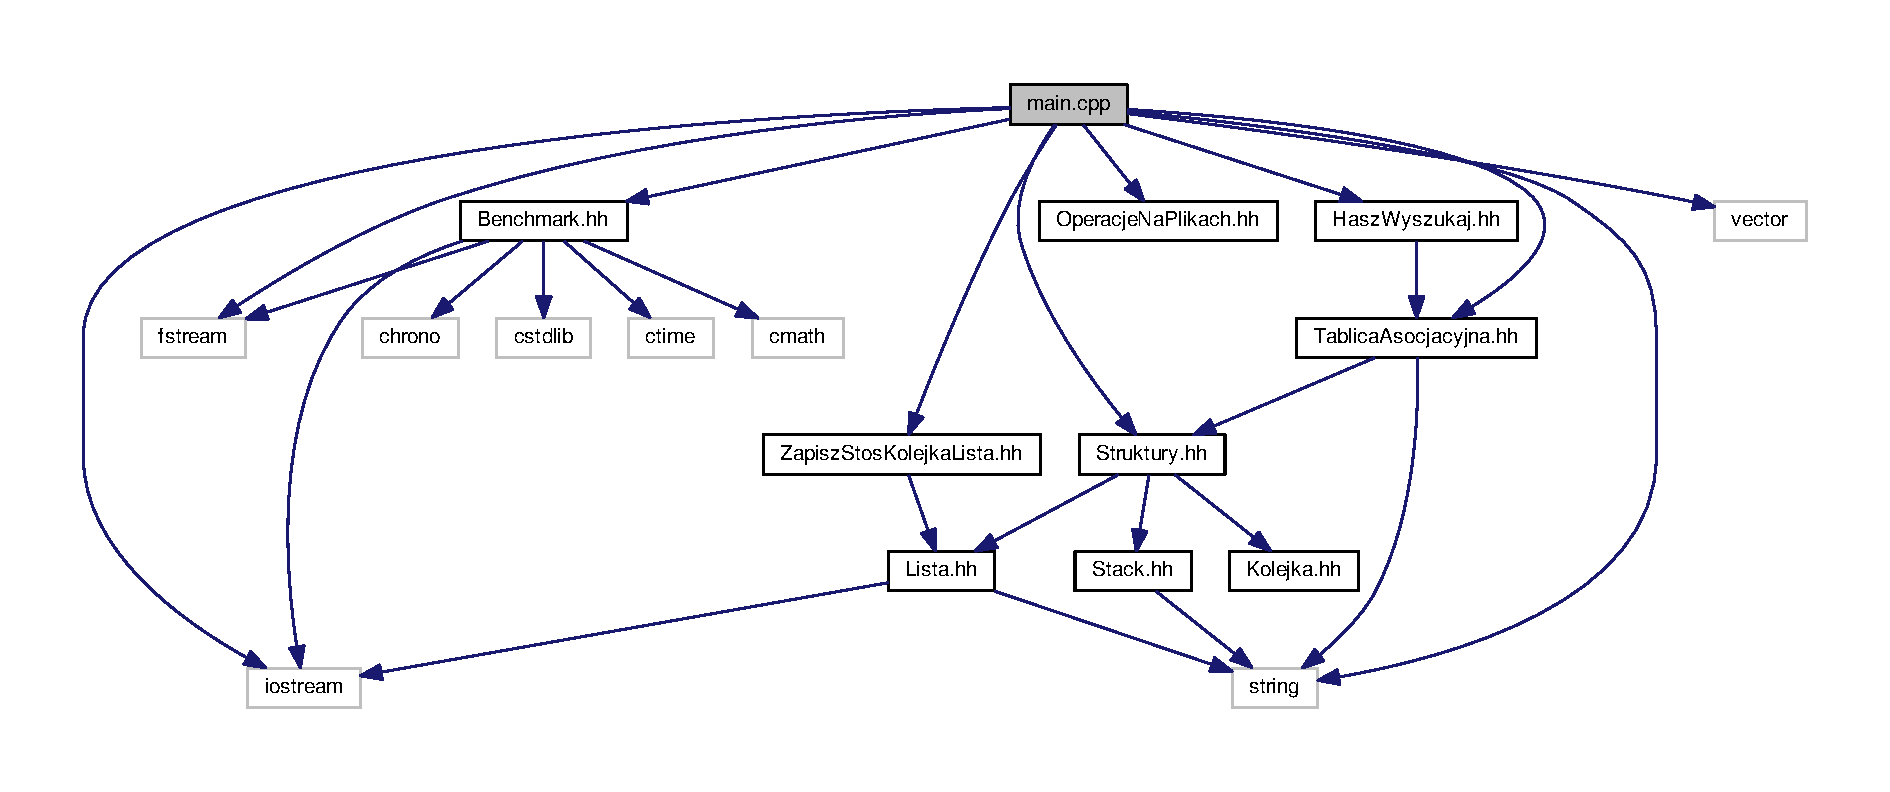
\includegraphics[width=350pt]{main_8cpp__incl}
\end{center}
\end{figure}
\subsection*{Funkcje}
\begin{DoxyCompactItemize}
\item 
int {\bf main} (int argc, char $\ast$argv[$\,$])
\end{DoxyCompactItemize}


\subsection{Dokumentacja funkcji}
\index{main.\-cpp@{main.\-cpp}!main@{main}}
\index{main@{main}!main.cpp@{main.\-cpp}}
\subsubsection[{main}]{\setlength{\rightskip}{0pt plus 5cm}int main (
\begin{DoxyParamCaption}
\item[{int}]{argc, }
\item[{char $\ast$}]{argv[$\,$]}
\end{DoxyParamCaption}
)}\label{main_8cpp_a0ddf1224851353fc92bfbff6f499fa97}


Definicja w linii 13 pliku main.\-cpp.



Oto graf wywołań dla tej funkcji\-:
\nopagebreak
\begin{figure}[H]
\begin{center}
\leavevmode
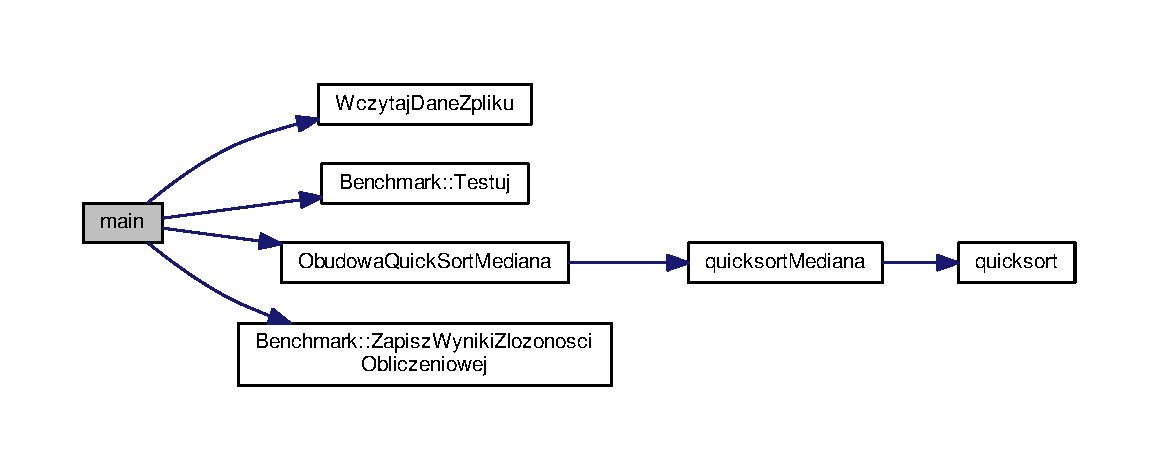
\includegraphics[width=350pt]{main_8cpp_a0ddf1224851353fc92bfbff6f499fa97_cgraph}
\end{center}
\end{figure}



\section{Dokumentacja pliku Node\-T.\-hh}
\label{_node_t_8hh}\index{Node\-T.\-hh@{Node\-T.\-hh}}
\subsection*{Komponenty}
\begin{DoxyCompactItemize}
\item 
class {\bf Node\-T$<$ Klucz, T $>$}
\end{DoxyCompactItemize}

\section{Dokumentacja pliku Operacje\-Na\-Plikach.\-hh}
\label{_operacje_na_plikach_8hh}\index{Operacje\-Na\-Plikach.\-hh@{Operacje\-Na\-Plikach.\-hh}}
Ten wykres pokazuje, które pliki bezpośrednio lub pośrednio załączają ten plik\-:
\nopagebreak
\begin{figure}[H]
\begin{center}
\leavevmode
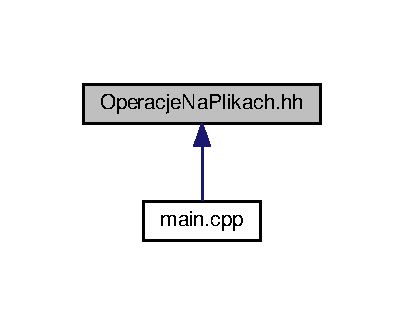
\includegraphics[width=216pt]{_operacje_na_plikach_8hh__dep__incl}
\end{center}
\end{figure}
\subsection*{Funkcje}
\begin{DoxyCompactItemize}
\item 
{\footnotesize template$<$typename T $>$ }\\std\-::istream \& {\bf Wczytaj\-Dane\-Zpliku} (std\-::istream \&Strm, unsigned long int Ilosc\-Danych, T $\ast$dane)
\end{DoxyCompactItemize}


\subsection{Dokumentacja funkcji}
\index{Operacje\-Na\-Plikach.\-hh@{Operacje\-Na\-Plikach.\-hh}!Wczytaj\-Dane\-Zpliku@{Wczytaj\-Dane\-Zpliku}}
\index{Wczytaj\-Dane\-Zpliku@{Wczytaj\-Dane\-Zpliku}!OperacjeNaPlikach.hh@{Operacje\-Na\-Plikach.\-hh}}
\subsubsection[{Wczytaj\-Dane\-Zpliku}]{\setlength{\rightskip}{0pt plus 5cm}template$<$typename T $>$ std\-::istream\& Wczytaj\-Dane\-Zpliku (
\begin{DoxyParamCaption}
\item[{std\-::istream \&}]{Strm, }
\item[{unsigned long int}]{Ilosc\-Danych, }
\item[{T $\ast$}]{dane}
\end{DoxyParamCaption}
)}\label{_operacje_na_plikach_8hh_a2f8a60c9e29287c0cf58fbd148385060}
Funkcja sluzy do wczytania elementow ze strumienia 
\begin{DoxyParams}[1]{Parametry}
\mbox{\tt in}  & {\em \&\-Strm-\/} & referencja do strumienia wejsciowego \\
\hline
 & {\em Ilosc\-Danych} & -\/ ilosc, jak wiele danych ma byc wczytane \\
\hline
 & {\em $\ast$dane} & -\/ wskaznik na strukture do ktorej beda wczytywane dane \\
\hline
\end{DoxyParams}
\begin{DoxyReturn}{Zwraca}
zwraca referencje do strumienia wejsciowego 
\end{DoxyReturn}


Definicja w linii 11 pliku Operacje\-Na\-Plikach.\-hh.



Oto graf wywoływań tej funkcji\-:
\nopagebreak
\begin{figure}[H]
\begin{center}
\leavevmode
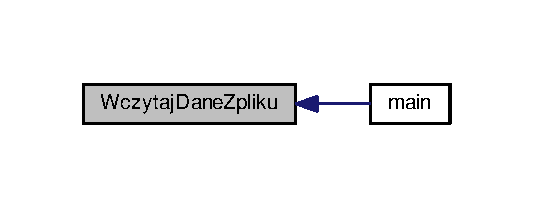
\includegraphics[width=256pt]{_operacje_na_plikach_8hh_a2f8a60c9e29287c0cf58fbd148385060_icgraph}
\end{center}
\end{figure}



\section{Dokumentacja pliku Sortowanie.\-cpp}
\label{_sortowanie_8cpp}\index{Sortowanie.\-cpp@{Sortowanie.\-cpp}}
{\ttfamily \#include \char`\"{}Sortowanie.\-hh\char`\"{}}\\*
Wykres zależności załączania dla Sortowanie.\-cpp\-:
\nopagebreak
\begin{figure}[H]
\begin{center}
\leavevmode
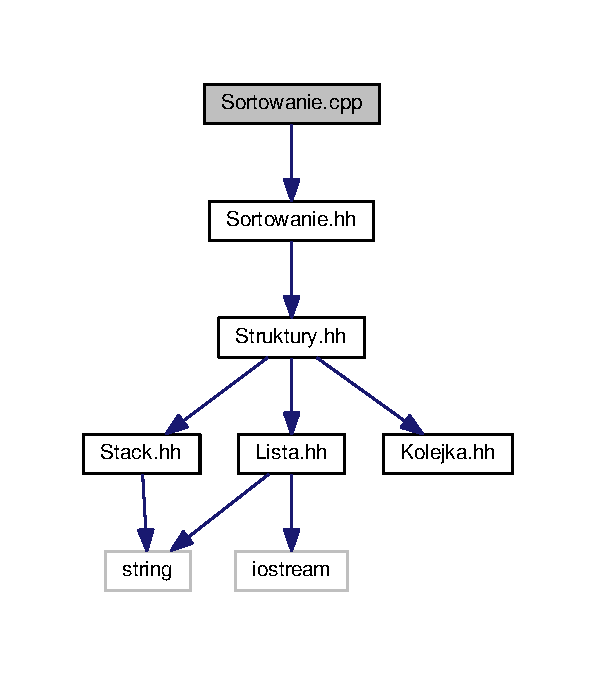
\includegraphics[width=286pt]{_sortowanie_8cpp__incl}
\end{center}
\end{figure}
\subsection*{Funkcje}
\begin{DoxyCompactItemize}
\item 
void {\bf quicksort} (int $\ast$tablica, int lewy, int prawy)
\item 
void {\bf Obudowa\-Quick\-Sort} (int $\ast$tablica, int rozmiar)
\item 
void {\bf quicksort\-Lista} ({\bf List}$<$ int $>$ $\ast$tablica, {\bf Node\-L}$<$ int $>$ $\ast$lewy, {\bf Node\-L}$<$ int $>$ $\ast$prawy, int index\-Lewy, int index\-Prawy)
\item 
void {\bf Ob} ({\bf List}$<$ int $>$ $\ast$list, int rozmiar)
\item 
void {\bf Merging} ({\bf Stack}$<$ int $>$ $\ast$tab, int lewy, int srodek, int prawy)
\item 
void {\bf Merge\-Sortowanie} ({\bf Stack}$<$ int $>$ $\ast$tab, int lewy, int prawy)
\end{DoxyCompactItemize}


\subsection{Dokumentacja funkcji}
\index{Sortowanie.\-cpp@{Sortowanie.\-cpp}!Merge\-Sortowanie@{Merge\-Sortowanie}}
\index{Merge\-Sortowanie@{Merge\-Sortowanie}!Sortowanie.cpp@{Sortowanie.\-cpp}}
\subsubsection[{Merge\-Sortowanie}]{\setlength{\rightskip}{0pt plus 5cm}void Merge\-Sortowanie (
\begin{DoxyParamCaption}
\item[{{\bf Stack}$<$ int $>$ $\ast$}]{tab, }
\item[{int}]{lewy, }
\item[{int}]{prawy}
\end{DoxyParamCaption}
)}\label{_sortowanie_8cpp_ab00f437616b519c083daf8fd32dc3c79}
brief Funkcja sortuje tablice skladajaca sie z elementow typu int za pomoca algorytmu Scalania 
\begin{DoxyParams}{Parametry}
{\em \mbox{]}} & tab-\/ typ Stack$<$int$>$ $\ast$, wskaznik na tablice do posortowania \\
\hline
{\em \mbox{]}} & lewy -\/ typ int, indeks poczatku lewej podtablicy \\
\hline
{\em \mbox{]}} & prawy -\/ typ int, indeks konca prawej podtablicy \\
\hline
\end{DoxyParams}


Definicja w linii 125 pliku Sortowanie.\-cpp.



Oto graf wywołań dla tej funkcji\-:
\nopagebreak
\begin{figure}[H]
\begin{center}
\leavevmode
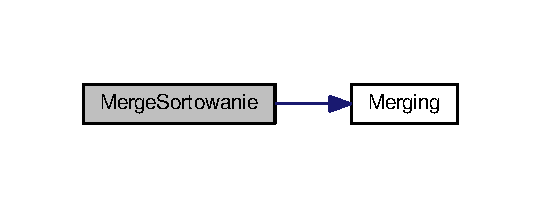
\includegraphics[width=260pt]{_sortowanie_8cpp_ab00f437616b519c083daf8fd32dc3c79_cgraph}
\end{center}
\end{figure}


\index{Sortowanie.\-cpp@{Sortowanie.\-cpp}!Merging@{Merging}}
\index{Merging@{Merging}!Sortowanie.cpp@{Sortowanie.\-cpp}}
\subsubsection[{Merging}]{\setlength{\rightskip}{0pt plus 5cm}void Merging (
\begin{DoxyParamCaption}
\item[{{\bf Stack}$<$ int $>$ $\ast$}]{tab, }
\item[{int}]{lewy, }
\item[{int}]{srodek, }
\item[{int}]{prawy}
\end{DoxyParamCaption}
)}\label{_sortowanie_8cpp_a0621dcd631e5d5c2ff4080e2106c06f1}
brief Funkcja scala dwa zbiory liczb rosnaca, jest funkcja skladowa Merge\-Sortowanie 
\begin{DoxyParams}{Parametry}
{\em \mbox{]}} & tab-\/ typ Stack$<$int$>$ $\ast$, wskaznik na tablice do scalenia \\
\hline
{\em \mbox{]}} & lewy -\/ typ int, indeks poczatku lewej podtablicy \\
\hline
{\em \mbox{]}} & srodek -\/typ int, indeks konca lewj podtablicy \\
\hline
{\em \mbox{]}} & prawy -\/ typ int, indeks konca prawej podtablicy \\
\hline
\end{DoxyParams}


Definicja w linii 98 pliku Sortowanie.\-cpp.



Oto graf wywoływań tej funkcji\-:
\nopagebreak
\begin{figure}[H]
\begin{center}
\leavevmode
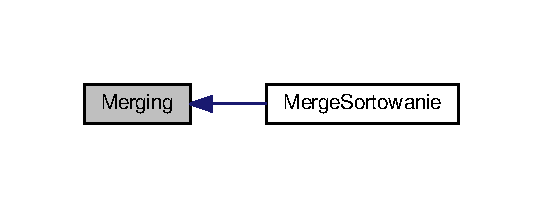
\includegraphics[width=260pt]{_sortowanie_8cpp_a0621dcd631e5d5c2ff4080e2106c06f1_icgraph}
\end{center}
\end{figure}


\index{Sortowanie.\-cpp@{Sortowanie.\-cpp}!Ob@{Ob}}
\index{Ob@{Ob}!Sortowanie.cpp@{Sortowanie.\-cpp}}
\subsubsection[{Ob}]{\setlength{\rightskip}{0pt plus 5cm}void Ob (
\begin{DoxyParamCaption}
\item[{{\bf List}$<$ int $>$ $\ast$}]{list, }
\item[{int}]{rozmiar}
\end{DoxyParamCaption}
)}\label{_sortowanie_8cpp_a08b237eec08c3e09ab1fae1f8bb1228a}
brief Funkcja obudowuje funkcje quicksort, zeby mogla zostac wczytana przez klase \doxyref{Benchmark}{str.}{class_benchmark} 
\begin{DoxyParams}{Parametry}
{\em \mbox{]}} & list -\/ typ List$<$int$>$$\ast$, wskaznik na liste do posortowania \\
\hline
{\em \mbox{]}} & rozmiar -\/ typ int, ilosc elementow do posortowania zaczynajac od poczatku listy \\
\hline
\end{DoxyParams}


Definicja w linii 82 pliku Sortowanie.\-cpp.



Oto graf wywołań dla tej funkcji\-:
\nopagebreak
\begin{figure}[H]
\begin{center}
\leavevmode
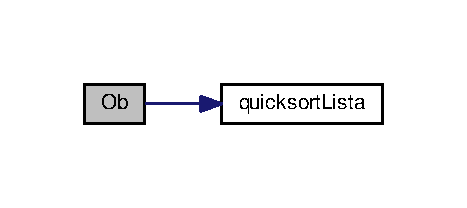
\includegraphics[width=224pt]{_sortowanie_8cpp_a08b237eec08c3e09ab1fae1f8bb1228a_cgraph}
\end{center}
\end{figure}


\index{Sortowanie.\-cpp@{Sortowanie.\-cpp}!Obudowa\-Quick\-Sort@{Obudowa\-Quick\-Sort}}
\index{Obudowa\-Quick\-Sort@{Obudowa\-Quick\-Sort}!Sortowanie.cpp@{Sortowanie.\-cpp}}
\subsubsection[{Obudowa\-Quick\-Sort}]{\setlength{\rightskip}{0pt plus 5cm}void Obudowa\-Quick\-Sort (
\begin{DoxyParamCaption}
\item[{int $\ast$}]{tablica, }
\item[{int}]{rozmiar}
\end{DoxyParamCaption}
)}\label{_sortowanie_8cpp_a5e829d34c4e1d2f4ce4d05c5f810e6cb}
brief Funkcja obudowuje funkcje quicksort, zeby mogla zostac wczytana przez klase \doxyref{Benchmark}{str.}{class_benchmark} 
\begin{DoxyParams}{Parametry}
{\em \mbox{]}} & tablica -\/ typ int$\ast$, wskaznik na tablice do posortowania \\
\hline
{\em \mbox{]}} & rozmiar -\/ typ int, ilosc elementow do posortowania zaczynajac od indeksu 0 \\
\hline
\end{DoxyParams}


Definicja w linii 38 pliku Sortowanie.\-cpp.



Oto graf wywołań dla tej funkcji\-:
\nopagebreak
\begin{figure}[H]
\begin{center}
\leavevmode
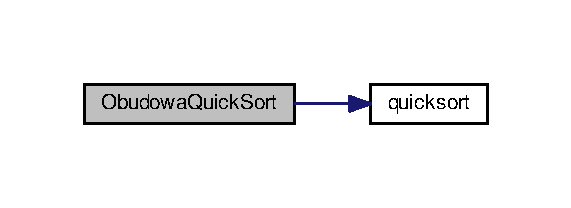
\includegraphics[width=274pt]{_sortowanie_8cpp_a5e829d34c4e1d2f4ce4d05c5f810e6cb_cgraph}
\end{center}
\end{figure}


\index{Sortowanie.\-cpp@{Sortowanie.\-cpp}!quicksort@{quicksort}}
\index{quicksort@{quicksort}!Sortowanie.cpp@{Sortowanie.\-cpp}}
\subsubsection[{quicksort}]{\setlength{\rightskip}{0pt plus 5cm}void quicksort (
\begin{DoxyParamCaption}
\item[{int $\ast$}]{tablica, }
\item[{int}]{lewy, }
\item[{int}]{prawy}
\end{DoxyParamCaption}
)}\label{_sortowanie_8cpp_afeb0867fa199171cc82cfb1c7db6c747}
Funkcja sortuje tablice typu int za pomoca algorytmu quicksort 
\begin{DoxyParams}{Parametry}
{\em \mbox{]}} & tablica -\/ typ int$\ast$, wskaznik na tablice do posortowania \\
\hline
{\em \mbox{]}} & lewy -\/ typ int, lewy indeks tablicy \\
\hline
{\em \mbox{]}} & prawy -\/ typ int, prawy indeks tablicy \\
\hline
\end{DoxyParams}


Definicja w linii 9 pliku Sortowanie.\-cpp.



Oto graf wywoływań tej funkcji\-:
\nopagebreak
\begin{figure}[H]
\begin{center}
\leavevmode
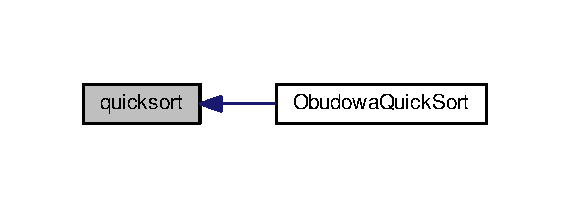
\includegraphics[width=274pt]{_sortowanie_8cpp_afeb0867fa199171cc82cfb1c7db6c747_icgraph}
\end{center}
\end{figure}


\index{Sortowanie.\-cpp@{Sortowanie.\-cpp}!quicksort\-Lista@{quicksort\-Lista}}
\index{quicksort\-Lista@{quicksort\-Lista}!Sortowanie.cpp@{Sortowanie.\-cpp}}
\subsubsection[{quicksort\-Lista}]{\setlength{\rightskip}{0pt plus 5cm}void quicksort\-Lista (
\begin{DoxyParamCaption}
\item[{{\bf List}$<$ int $>$ $\ast$}]{tablica, }
\item[{{\bf Node\-L}$<$ int $>$ $\ast$}]{lewy, }
\item[{{\bf Node\-L}$<$ int $>$ $\ast$}]{prawy, }
\item[{int}]{index\-Lewy, }
\item[{int}]{index\-Prawy}
\end{DoxyParamCaption}
)}\label{_sortowanie_8cpp_af467a7de462587952ddc60c3fc097d06}
Funkcja sortuje Liste skladajaca sie z elementow typu int za pomoca algorytmu quicksort 
\begin{DoxyParams}{Parametry}
{\em \mbox{]}} & tablica -\/ typ List$<$int$>$$\ast$, wskaznik na Liste do posortowania \\
\hline
{\em \mbox{]}} & lewy -\/ Node\-L$<$int$>$ $\ast$ ,wskaznik na lewy wezel Listy \\
\hline
{\em \mbox{]}} & prawy -\/ Node\-L$<$int$>$ $\ast$, wskaznik na prawy wezel Listy \\
\hline
\end{DoxyParams}


Definicja w linii 51 pliku Sortowanie.\-cpp.



Oto graf wywoływań tej funkcji\-:
\nopagebreak
\begin{figure}[H]
\begin{center}
\leavevmode
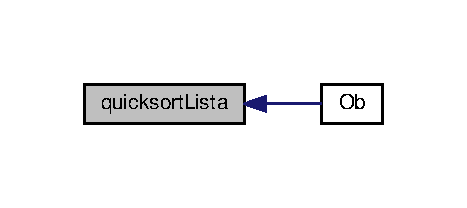
\includegraphics[width=224pt]{_sortowanie_8cpp_af467a7de462587952ddc60c3fc097d06_icgraph}
\end{center}
\end{figure}



\section{Dokumentacja pliku Sortowanie.\-hh}
\label{_sortowanie_8hh}\index{Sortowanie.\-hh@{Sortowanie.\-hh}}
{\ttfamily \#include \char`\"{}Struktury.\-hh\char`\"{}}\\*
Wykres zależności załączania dla Sortowanie.\-hh\-:
\nopagebreak
\begin{figure}[H]
\begin{center}
\leavevmode
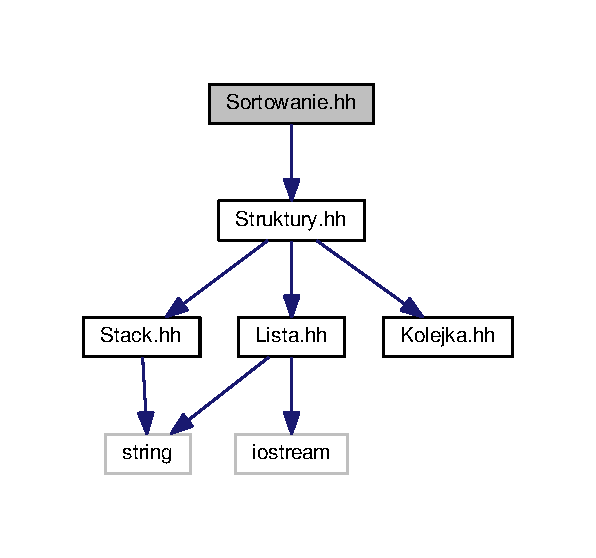
\includegraphics[width=286pt]{_sortowanie_8hh__incl}
\end{center}
\end{figure}
Ten wykres pokazuje, które pliki bezpośrednio lub pośrednio załączają ten plik\-:
\nopagebreak
\begin{figure}[H]
\begin{center}
\leavevmode
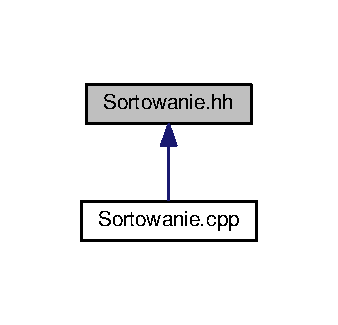
\includegraphics[width=162pt]{_sortowanie_8hh__dep__incl}
\end{center}
\end{figure}
\subsection*{Funkcje}
\begin{DoxyCompactItemize}
\item 
void {\bf quicksort} (int $\ast$tablica, int lewy, int prawy)
\item 
void {\bf Obudowa\-Quick\-Sort} (int $\ast$tablica, int rozmiar)
\item 
void {\bf quicksort\-Lista} ({\bf List}$<$ int $>$ $\ast$tablica, {\bf Node\-L}$<$ int $>$ $\ast$lewy, {\bf Node\-L}$<$ int $>$ $\ast$prawy, int l, int p)
\item 
void {\bf Ob} ({\bf List}$<$ int $>$ $\ast$tablica, int rozmiar)
\item 
void {\bf Merge\-Sortowanie} ({\bf Stack}$<$ int $>$ $\ast$tablica, int lewy, int prawy)
\item 
void {\bf Merging} ({\bf Stack}$<$ int $>$ $\ast$tablica, int lewy, int srodkowy, int prawy)
\end{DoxyCompactItemize}


\subsection{Dokumentacja funkcji}
\index{Sortowanie.\-hh@{Sortowanie.\-hh}!Merge\-Sortowanie@{Merge\-Sortowanie}}
\index{Merge\-Sortowanie@{Merge\-Sortowanie}!Sortowanie.hh@{Sortowanie.\-hh}}
\subsubsection[{Merge\-Sortowanie}]{\setlength{\rightskip}{0pt plus 5cm}void Merge\-Sortowanie (
\begin{DoxyParamCaption}
\item[{{\bf Stack}$<$ int $>$ $\ast$}]{tab, }
\item[{int}]{lewy, }
\item[{int}]{prawy}
\end{DoxyParamCaption}
)}\label{_sortowanie_8hh_a2f2eed0a21e81ccef5be0ac4e4e025b2}
brief Funkcja sortuje tablice skladajaca sie z elementow typu int za pomoca algorytmu Scalania

brief Funkcja sortuje tablice skladajaca sie z elementow typu int za pomoca algorytmu Scalania 
\begin{DoxyParams}{Parametry}
{\em \mbox{]}} & tab-\/ typ Stack$<$int$>$ $\ast$, wskaznik na tablice do posortowania \\
\hline
{\em \mbox{]}} & lewy -\/ typ int, indeks poczatku lewej podtablicy \\
\hline
{\em \mbox{]}} & prawy -\/ typ int, indeks konca prawej podtablicy \\
\hline
\end{DoxyParams}


Definicja w linii 125 pliku Sortowanie.\-cpp.



Oto graf wywołań dla tej funkcji\-:
\nopagebreak
\begin{figure}[H]
\begin{center}
\leavevmode
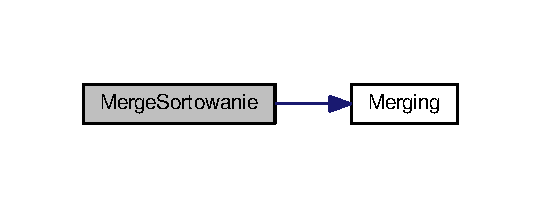
\includegraphics[width=260pt]{_sortowanie_8hh_a2f2eed0a21e81ccef5be0ac4e4e025b2_cgraph}
\end{center}
\end{figure}


\index{Sortowanie.\-hh@{Sortowanie.\-hh}!Merging@{Merging}}
\index{Merging@{Merging}!Sortowanie.hh@{Sortowanie.\-hh}}
\subsubsection[{Merging}]{\setlength{\rightskip}{0pt plus 5cm}void Merging (
\begin{DoxyParamCaption}
\item[{{\bf Stack}$<$ int $>$ $\ast$}]{tab, }
\item[{int}]{lewy, }
\item[{int}]{srodek, }
\item[{int}]{prawy}
\end{DoxyParamCaption}
)}\label{_sortowanie_8hh_a1860ac02082a0b636ce2623b03a0f08d}
brief Funkcja scala dwa zbiory liczb, jest funkcja skladowa Merge\-Sortowanie

brief Funkcja scala dwa zbiory liczb rosnaca, jest funkcja skladowa Merge\-Sortowanie 
\begin{DoxyParams}{Parametry}
{\em \mbox{]}} & tab-\/ typ Stack$<$int$>$ $\ast$, wskaznik na tablice do scalenia \\
\hline
{\em \mbox{]}} & lewy -\/ typ int, indeks poczatku lewej podtablicy \\
\hline
{\em \mbox{]}} & srodek -\/typ int, indeks konca lewj podtablicy \\
\hline
{\em \mbox{]}} & prawy -\/ typ int, indeks konca prawej podtablicy \\
\hline
\end{DoxyParams}


Definicja w linii 98 pliku Sortowanie.\-cpp.



Oto graf wywoływań tej funkcji\-:
\nopagebreak
\begin{figure}[H]
\begin{center}
\leavevmode
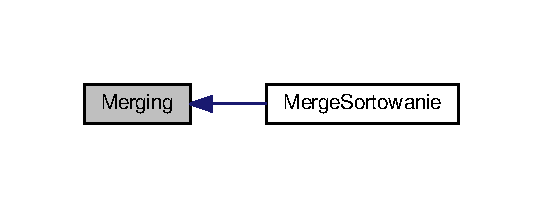
\includegraphics[width=260pt]{_sortowanie_8hh_a1860ac02082a0b636ce2623b03a0f08d_icgraph}
\end{center}
\end{figure}


\index{Sortowanie.\-hh@{Sortowanie.\-hh}!Ob@{Ob}}
\index{Ob@{Ob}!Sortowanie.hh@{Sortowanie.\-hh}}
\subsubsection[{Ob}]{\setlength{\rightskip}{0pt plus 5cm}void Ob (
\begin{DoxyParamCaption}
\item[{{\bf List}$<$ int $>$ $\ast$}]{list, }
\item[{int}]{rozmiar}
\end{DoxyParamCaption}
)}\label{_sortowanie_8hh_aa2e09d4d5398e34076a4b3fa6779c8d5}
brief Funkcja obudowuje funkcje quicksort\-Lista,zeby mogla zostac wczytana przez klase \doxyref{Benchmark}{str.}{class_benchmark}

brief Funkcja obudowuje funkcje quicksort, zeby mogla zostac wczytana przez klase \doxyref{Benchmark}{str.}{class_benchmark} 
\begin{DoxyParams}{Parametry}
{\em \mbox{]}} & list -\/ typ List$<$int$>$$\ast$, wskaznik na liste do posortowania \\
\hline
{\em \mbox{]}} & rozmiar -\/ typ int, ilosc elementow do posortowania zaczynajac od poczatku listy \\
\hline
\end{DoxyParams}


Definicja w linii 82 pliku Sortowanie.\-cpp.



Oto graf wywołań dla tej funkcji\-:
\nopagebreak
\begin{figure}[H]
\begin{center}
\leavevmode
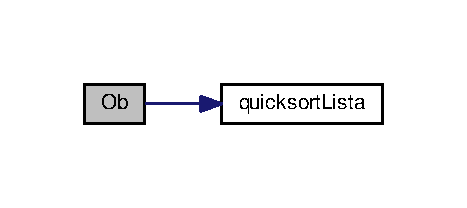
\includegraphics[width=224pt]{_sortowanie_8hh_aa2e09d4d5398e34076a4b3fa6779c8d5_cgraph}
\end{center}
\end{figure}


\index{Sortowanie.\-hh@{Sortowanie.\-hh}!Obudowa\-Quick\-Sort@{Obudowa\-Quick\-Sort}}
\index{Obudowa\-Quick\-Sort@{Obudowa\-Quick\-Sort}!Sortowanie.hh@{Sortowanie.\-hh}}
\subsubsection[{Obudowa\-Quick\-Sort}]{\setlength{\rightskip}{0pt plus 5cm}void Obudowa\-Quick\-Sort (
\begin{DoxyParamCaption}
\item[{int $\ast$}]{tablica, }
\item[{int}]{rozmiar}
\end{DoxyParamCaption}
)}\label{_sortowanie_8hh_a5e829d34c4e1d2f4ce4d05c5f810e6cb}
brief Funkcja obudowuje funkcje quicksort, zeby mogla zostac wczytana przez klase \doxyref{Benchmark}{str.}{class_benchmark}

brief Funkcja obudowuje funkcje quicksort, zeby mogla zostac wczytana przez klase \doxyref{Benchmark}{str.}{class_benchmark} 
\begin{DoxyParams}{Parametry}
{\em \mbox{]}} & tablica -\/ typ int$\ast$, wskaznik na tablice do posortowania \\
\hline
{\em \mbox{]}} & rozmiar -\/ typ int, ilosc elementow do posortowania zaczynajac od indeksu 0 \\
\hline
\end{DoxyParams}


Definicja w linii 38 pliku Sortowanie.\-cpp.



Oto graf wywołań dla tej funkcji\-:
\nopagebreak
\begin{figure}[H]
\begin{center}
\leavevmode
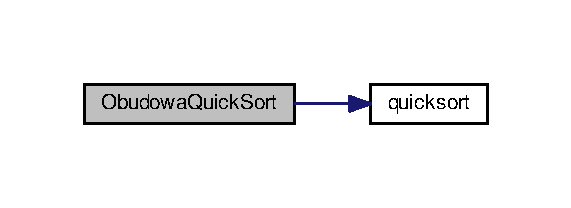
\includegraphics[width=274pt]{_sortowanie_8hh_a5e829d34c4e1d2f4ce4d05c5f810e6cb_cgraph}
\end{center}
\end{figure}


\index{Sortowanie.\-hh@{Sortowanie.\-hh}!quicksort@{quicksort}}
\index{quicksort@{quicksort}!Sortowanie.hh@{Sortowanie.\-hh}}
\subsubsection[{quicksort}]{\setlength{\rightskip}{0pt plus 5cm}void quicksort (
\begin{DoxyParamCaption}
\item[{int $\ast$}]{tablica, }
\item[{int}]{lewy, }
\item[{int}]{prawy}
\end{DoxyParamCaption}
)}\label{_sortowanie_8hh_afeb0867fa199171cc82cfb1c7db6c747}
brief Funkcja sortuje tablice typu int za pomoca algorytmu quicksort

Funkcja sortuje tablice typu int za pomoca algorytmu quicksort 
\begin{DoxyParams}{Parametry}
{\em \mbox{]}} & tablica -\/ typ int$\ast$, wskaznik na tablice do posortowania \\
\hline
{\em \mbox{]}} & lewy -\/ typ int, lewy indeks tablicy \\
\hline
{\em \mbox{]}} & prawy -\/ typ int, prawy indeks tablicy \\
\hline
\end{DoxyParams}


Definicja w linii 9 pliku Sortowanie.\-cpp.



Oto graf wywoływań tej funkcji\-:
\nopagebreak
\begin{figure}[H]
\begin{center}
\leavevmode
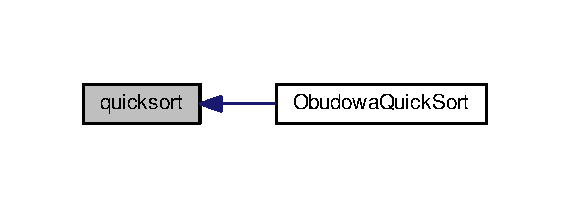
\includegraphics[width=274pt]{_sortowanie_8hh_afeb0867fa199171cc82cfb1c7db6c747_icgraph}
\end{center}
\end{figure}


\index{Sortowanie.\-hh@{Sortowanie.\-hh}!quicksort\-Lista@{quicksort\-Lista}}
\index{quicksort\-Lista@{quicksort\-Lista}!Sortowanie.hh@{Sortowanie.\-hh}}
\subsubsection[{quicksort\-Lista}]{\setlength{\rightskip}{0pt plus 5cm}void quicksort\-Lista (
\begin{DoxyParamCaption}
\item[{{\bf List}$<$ int $>$ $\ast$}]{tablica, }
\item[{{\bf Node\-L}$<$ int $>$ $\ast$}]{lewy, }
\item[{{\bf Node\-L}$<$ int $>$ $\ast$}]{prawy, }
\item[{int}]{index\-Lewy, }
\item[{int}]{index\-Prawy}
\end{DoxyParamCaption}
)}\label{_sortowanie_8hh_a42f1c935498843da7fbaf94f71b1177e}
brief Funkcja sortuje Liste skladajace sie z elementow typu int za pomoca algorytmu quicksort

Funkcja sortuje Liste skladajaca sie z elementow typu int za pomoca algorytmu quicksort 
\begin{DoxyParams}{Parametry}
{\em \mbox{]}} & tablica -\/ typ List$<$int$>$$\ast$, wskaznik na Liste do posortowania \\
\hline
{\em \mbox{]}} & lewy -\/ Node\-L$<$int$>$ $\ast$ ,wskaznik na lewy wezel Listy \\
\hline
{\em \mbox{]}} & prawy -\/ Node\-L$<$int$>$ $\ast$, wskaznik na prawy wezel Listy \\
\hline
\end{DoxyParams}


Definicja w linii 51 pliku Sortowanie.\-cpp.



Oto graf wywoływań tej funkcji\-:
\nopagebreak
\begin{figure}[H]
\begin{center}
\leavevmode
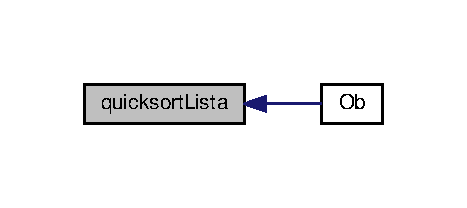
\includegraphics[width=224pt]{_sortowanie_8hh_a42f1c935498843da7fbaf94f71b1177e_icgraph}
\end{center}
\end{figure}



\section{Dokumentacja pliku Stack.\-hh}
\label{_stack_8hh}\index{Stack.\-hh@{Stack.\-hh}}


Klasa \doxyref{Stack}{str.}{class_stack} sluzy do przechowywania, dodawania,zdejmowania kolejnych elementow stosu.  


{\ttfamily \#include $<$string$>$}\\*
Wykres zależności załączania dla Stack.\-hh\-:
\nopagebreak
\begin{figure}[H]
\begin{center}
\leavevmode
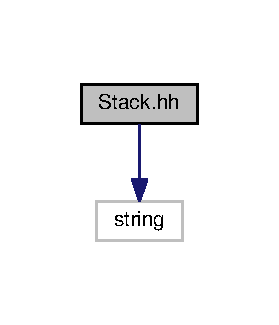
\includegraphics[width=134pt]{_stack_8hh__incl}
\end{center}
\end{figure}
Ten wykres pokazuje, które pliki bezpośrednio lub pośrednio załączają ten plik\-:
\nopagebreak
\begin{figure}[H]
\begin{center}
\leavevmode
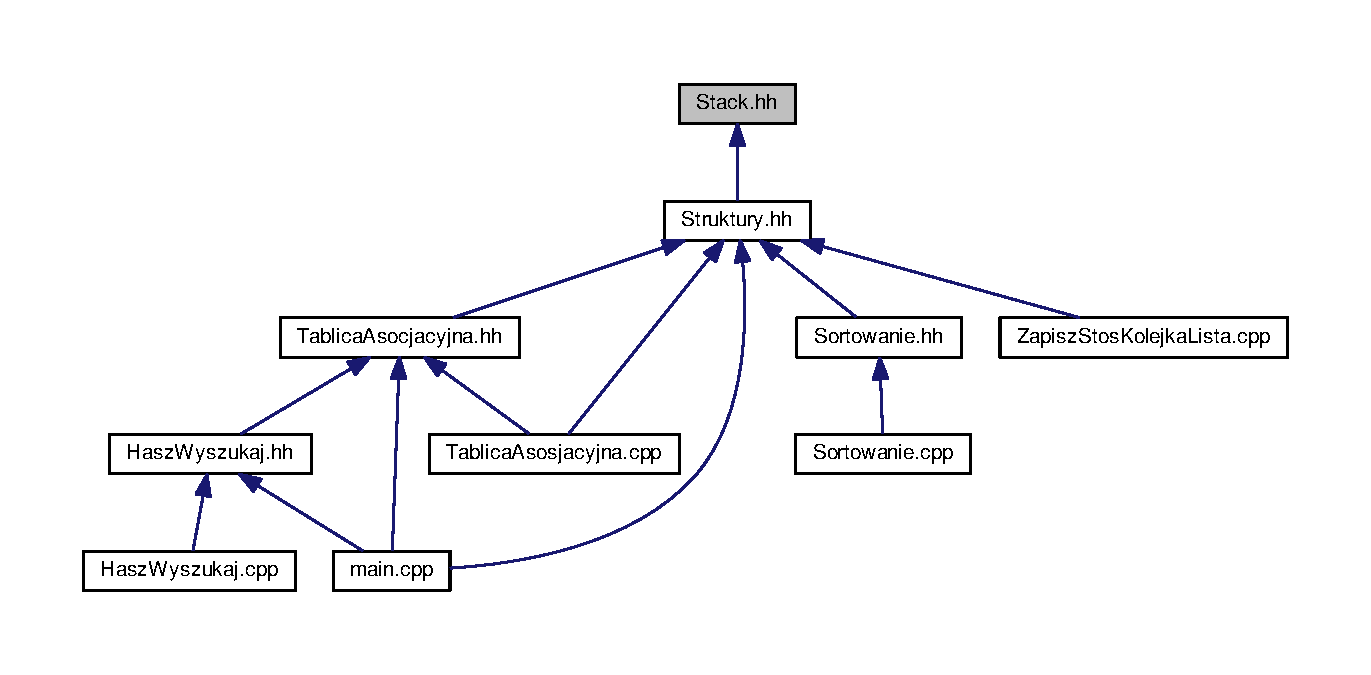
\includegraphics[width=350pt]{_stack_8hh__dep__incl}
\end{center}
\end{figure}
\subsection*{Komponenty}
\begin{DoxyCompactItemize}
\item 
class {\bf Stack$<$ T $>$}
\end{DoxyCompactItemize}
\subsection*{Funkcje}
\begin{DoxyCompactItemize}
\item 
{\footnotesize template$<$typename T $>$ }\\std\-::ostream \& {\bf operator$<$$<$} (std\-::ostream \&out, const {\bf Stack}$<$ T $>$ \&stack)
\end{DoxyCompactItemize}


\subsection{Dokumentacja funkcji}
\index{Stack.\-hh@{Stack.\-hh}!operator$<$$<$@{operator$<$$<$}}
\index{operator$<$$<$@{operator$<$$<$}!Stack.hh@{Stack.\-hh}}
\subsubsection[{operator$<$$<$}]{\setlength{\rightskip}{0pt plus 5cm}template$<$typename T $>$ std\-::ostream\& operator$<$$<$ (
\begin{DoxyParamCaption}
\item[{std\-::ostream \&}]{out, }
\item[{const {\bf Stack}$<$ T $>$ \&}]{stack}
\end{DoxyParamCaption}
)}\label{_stack_8hh_a3a3ec1f00086320ead07a87074476e81}
Funkcja operatorowa sluzy do wyswietlania stosu,zbedna 
\begin{DoxyParams}[1]{Parametry}
\mbox{\tt in}  & {\em \&out} & -\/ referencja do strumienia wyjsciowego \\
\hline
\mbox{\tt in}  & {\em \&stack-\/} & referencja do stosu \\
\hline
\end{DoxyParams}
\begin{DoxyReturn}{Zwraca}
zwraca referencje do strumienia wyjsciowego 
\end{DoxyReturn}


Definicja w linii 151 pliku Stack.\-hh.


\section{Dokumentacja pliku Struktury.\-hh}
\label{_struktury_8hh}\index{Struktury.\-hh@{Struktury.\-hh}}
{\ttfamily \#include \char`\"{}Stack.\-hh\char`\"{}}\\*
{\ttfamily \#include \char`\"{}Lista.\-hh\char`\"{}}\\*
{\ttfamily \#include \char`\"{}Kolejka.\-hh\char`\"{}}\\*
Wykres zależności załączania dla Struktury.\-hh\-:\nopagebreak
\begin{figure}[H]
\begin{center}
\leavevmode
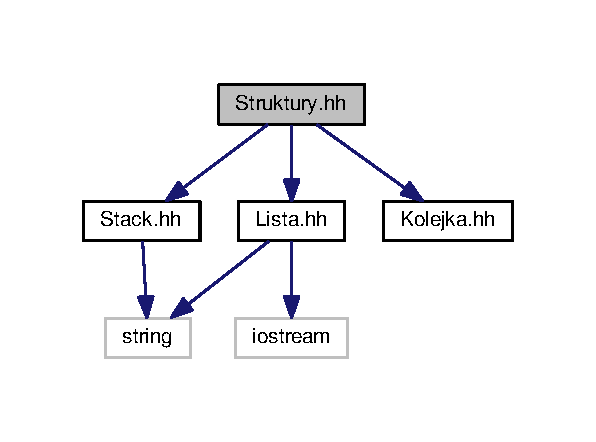
\includegraphics[width=286pt]{_struktury_8hh__incl}
\end{center}
\end{figure}
Ten wykres pokazuje, które pliki bezpośrednio lub pośrednio załączają ten plik\-:\nopagebreak
\begin{figure}[H]
\begin{center}
\leavevmode
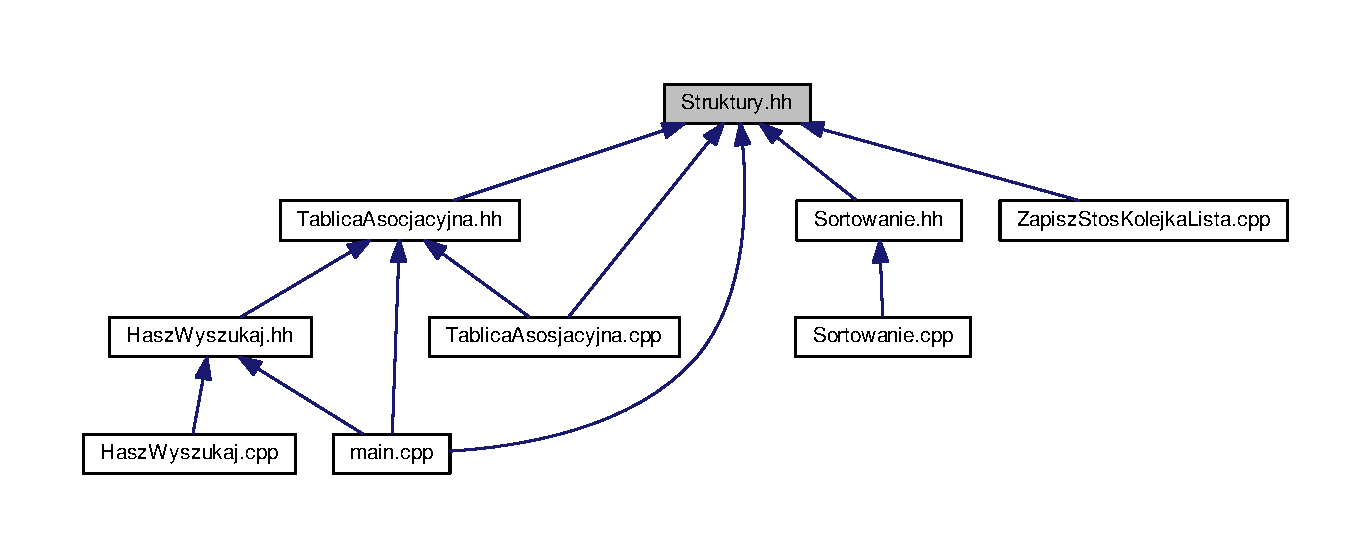
\includegraphics[width=218pt]{_struktury_8hh__dep__incl}
\end{center}
\end{figure}

\section{Dokumentacja pliku Tablica\-Asocjacyjna.\-hh}
\label{_tablica_asocjacyjna_8hh}\index{Tablica\-Asocjacyjna.\-hh@{Tablica\-Asocjacyjna.\-hh}}


Klasa \doxyref{Tablica\-Asocjacyjna}{str.}{class_tablica_asocjacyjna} sluzy do wykonywania zapisywania i wyszukiwania elementow z wykorzystaniem haszowania.  


{\ttfamily \#include $<$string$>$}\\*
{\ttfamily \#include \char`\"{}Struktury.\-hh\char`\"{}}\\*
Wykres zależności załączania dla Tablica\-Asocjacyjna.\-hh\-:
\nopagebreak
\begin{figure}[H]
\begin{center}
\leavevmode
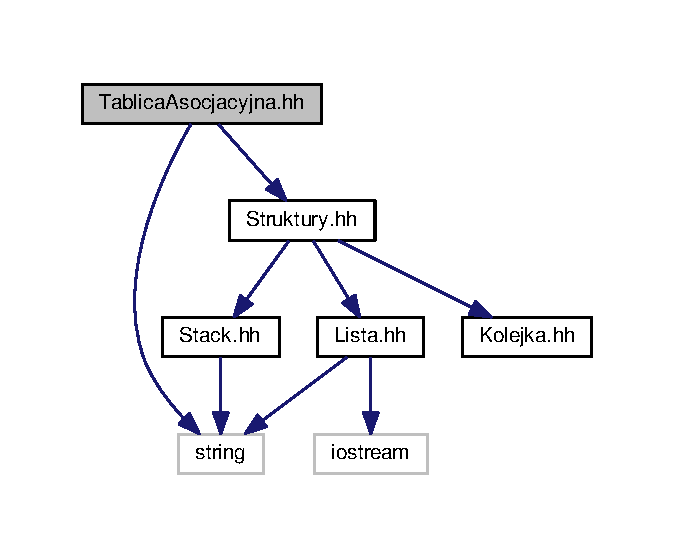
\includegraphics[width=324pt]{_tablica_asocjacyjna_8hh__incl}
\end{center}
\end{figure}
Ten wykres pokazuje, które pliki bezpośrednio lub pośrednio załączają ten plik\-:
\nopagebreak
\begin{figure}[H]
\begin{center}
\leavevmode
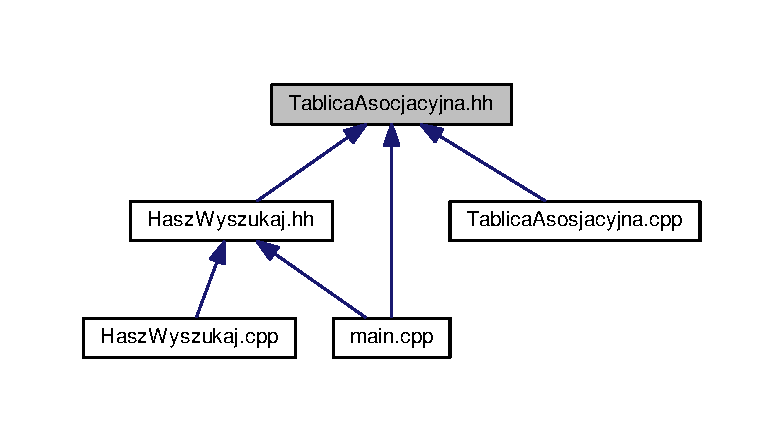
\includegraphics[width=350pt]{_tablica_asocjacyjna_8hh__dep__incl}
\end{center}
\end{figure}
\subsection*{Komponenty}
\begin{DoxyCompactItemize}
\item 
class {\bf Tablica\-Asocjacyjna}
\end{DoxyCompactItemize}

\section{Dokumentacja pliku Tablica\-Asosjacyjna.\-cpp}
\label{_tablica_asosjacyjna_8cpp}\index{Tablica\-Asosjacyjna.\-cpp@{Tablica\-Asosjacyjna.\-cpp}}
{\ttfamily \#include \char`\"{}Tablica\-Asocjacyjna.\-hh\char`\"{}}\\*
{\ttfamily \#include $<$string$>$}\\*
{\ttfamily \#include $<$iostream$>$}\\*
{\ttfamily \#include $<$Struktury.\-hh$>$}\\*
{\ttfamily \#include $<$sstream$>$}\\*
{\ttfamily \#include $<$fstream$>$}\\*
Wykres zależności załączania dla Tablica\-Asosjacyjna.\-cpp\-:
\nopagebreak
\begin{figure}[H]
\begin{center}
\leavevmode
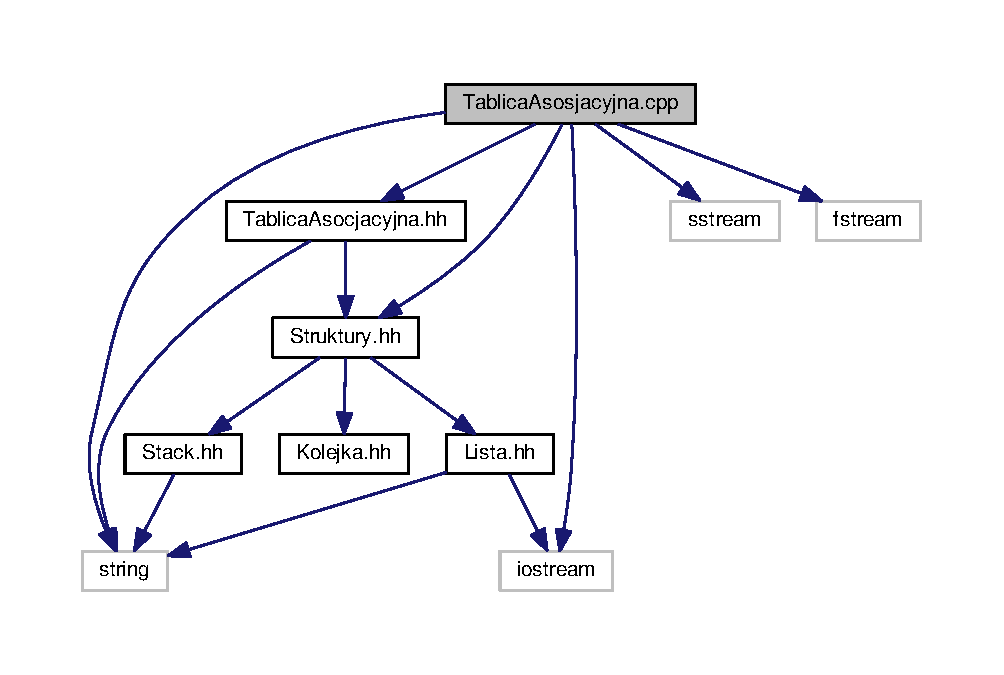
\includegraphics[width=350pt]{_tablica_asosjacyjna_8cpp__incl}
\end{center}
\end{figure}

\section{Dokumentacja pliku Zapisz\-Stos\-Kolejka\-Lista.\-cpp}
\label{_zapisz_stos_kolejka_lista_8cpp}\index{Zapisz\-Stos\-Kolejka\-Lista.\-cpp@{Zapisz\-Stos\-Kolejka\-Lista.\-cpp}}
{\ttfamily \#include $<$string$>$}\\*
{\ttfamily \#include $<$iostream$>$}\\*
{\ttfamily \#include \char`\"{}Struktury.\-hh\char`\"{}}\\*
{\ttfamily \#include \char`\"{}Zapisz\-Stos\-Kolejka\-Lista.\-hh\char`\"{}}\\*
Wykres zależności załączania dla Zapisz\-Stos\-Kolejka\-Lista.\-cpp\-:
\nopagebreak
\begin{figure}[H]
\begin{center}
\leavevmode
\includegraphics[width=349pt]{_zapisz_stos_kolejka_lista_8cpp__incl}
\end{center}
\end{figure}
\subsection*{Funkcje}
\begin{DoxyCompactItemize}
\item 
void {\bf Zapisz\-Kolejno\-Liczby\-Stosu} (double $\ast$Gausowe, int size)
\item 
void {\bf Zapisz\-Kolejno\-Liczby\-Listy} (double $\ast$Gausowe, int size)
\item 
void {\bf Zapisz\-Kolejno\-Liczby\-Kolejki} (double $\ast$Gausowe, int size)
\item 
void {\bf Wczytaj\-Liste} (std\-::istream \&Strm, unsigned long int Ilosc\-Danych, {\bf List}$<$ int $>$ $\ast$dane)
\end{DoxyCompactItemize}


\subsection{Dokumentacja funkcji}
\index{Zapisz\-Stos\-Kolejka\-Lista.\-cpp@{Zapisz\-Stos\-Kolejka\-Lista.\-cpp}!Wczytaj\-Liste@{Wczytaj\-Liste}}
\index{Wczytaj\-Liste@{Wczytaj\-Liste}!ZapiszStosKolejkaLista.cpp@{Zapisz\-Stos\-Kolejka\-Lista.\-cpp}}
\subsubsection[{Wczytaj\-Liste}]{\setlength{\rightskip}{0pt plus 5cm}void Wczytaj\-Liste (
\begin{DoxyParamCaption}
\item[{std\-::istream \&}]{Strm, }
\item[{unsigned long int}]{Ilosc\-Danych, }
\item[{{\bf List}$<$ int $>$ $\ast$}]{dane}
\end{DoxyParamCaption}
)}\label{_zapisz_stos_kolejka_lista_8cpp_a73d3a7f9c1a1106d9c4bd29f47b284b0}
brief Funkcja sluzy do Wczytania Listy o elementach typu int 
\begin{DoxyParams}{Parametry}
{\em \mbox{]}} & Strm -\/ referencja do strumienia wejsciowego \\
\hline
{\em \mbox{]}} & Ilosc\-Danych -\/ typ int, oznacza jak wiele danych ma byc wczytane \\
\hline
{\em \mbox{]}} & dane -\/ typ List$<$int$>$$\ast$, lista gdzie beda wczytane dane \\
\hline
\end{DoxyParams}


Definicja w linii 50 pliku Zapisz\-Stos\-Kolejka\-Lista.\-cpp.



Oto graf wywołań dla tej funkcji\-:
\nopagebreak
\begin{figure}[H]
\begin{center}
\leavevmode
\includegraphics[width=274pt]{_zapisz_stos_kolejka_lista_8cpp_a73d3a7f9c1a1106d9c4bd29f47b284b0_cgraph}
\end{center}
\end{figure}


\index{Zapisz\-Stos\-Kolejka\-Lista.\-cpp@{Zapisz\-Stos\-Kolejka\-Lista.\-cpp}!Zapisz\-Kolejno\-Liczby\-Kolejki@{Zapisz\-Kolejno\-Liczby\-Kolejki}}
\index{Zapisz\-Kolejno\-Liczby\-Kolejki@{Zapisz\-Kolejno\-Liczby\-Kolejki}!ZapiszStosKolejkaLista.cpp@{Zapisz\-Stos\-Kolejka\-Lista.\-cpp}}
\subsubsection[{Zapisz\-Kolejno\-Liczby\-Kolejki}]{\setlength{\rightskip}{0pt plus 5cm}void Zapisz\-Kolejno\-Liczby\-Kolejki (
\begin{DoxyParamCaption}
\item[{double $\ast$}]{Gausowe, }
\item[{int}]{size}
\end{DoxyParamCaption}
)}\label{_zapisz_stos_kolejka_lista_8cpp_a4ebb87eefdad7cefd386dd4888e26e3d}
Funkcja sluzy do zapisywania danych na Kolejce utworzonej w tej funkcji 
\begin{DoxyParams}{Parametry}
{\em \mbox{]}} & Gausowe -\/ typ double $\ast$, wskaznik na tablice typu double \\
\hline
{\em \mbox{]}} & size -\/ rozmiar, jak wiele liczb ma byc zapisane \\
\hline
\end{DoxyParams}


Definicja w linii 37 pliku Zapisz\-Stos\-Kolejka\-Lista.\-cpp.



Oto graf wywołań dla tej funkcji\-:
\nopagebreak
\begin{figure}[H]
\begin{center}
\leavevmode
\includegraphics[width=350pt]{_zapisz_stos_kolejka_lista_8cpp_a4ebb87eefdad7cefd386dd4888e26e3d_cgraph}
\end{center}
\end{figure}


\index{Zapisz\-Stos\-Kolejka\-Lista.\-cpp@{Zapisz\-Stos\-Kolejka\-Lista.\-cpp}!Zapisz\-Kolejno\-Liczby\-Listy@{Zapisz\-Kolejno\-Liczby\-Listy}}
\index{Zapisz\-Kolejno\-Liczby\-Listy@{Zapisz\-Kolejno\-Liczby\-Listy}!ZapiszStosKolejkaLista.cpp@{Zapisz\-Stos\-Kolejka\-Lista.\-cpp}}
\subsubsection[{Zapisz\-Kolejno\-Liczby\-Listy}]{\setlength{\rightskip}{0pt plus 5cm}void Zapisz\-Kolejno\-Liczby\-Listy (
\begin{DoxyParamCaption}
\item[{double $\ast$}]{Gausowe, }
\item[{int}]{size}
\end{DoxyParamCaption}
)}\label{_zapisz_stos_kolejka_lista_8cpp_a244eeea8d930f965ca549790df4fee65}
Funkcja sluzy do zapisywania danych na liscie utworzonej w tej funkcji 
\begin{DoxyParams}{Parametry}
{\em \mbox{]}} & Gausowe -\/ typ double $\ast$, wskaznik na tablice typu double \\
\hline
{\em \mbox{]}} & size -\/ rozmiar, jak wiele liczb ma byc zapisane \\
\hline
\end{DoxyParams}


Definicja w linii 25 pliku Zapisz\-Stos\-Kolejka\-Lista.\-cpp.



Oto graf wywołań dla tej funkcji\-:
\nopagebreak
\begin{figure}[H]
\begin{center}
\leavevmode
\includegraphics[width=330pt]{_zapisz_stos_kolejka_lista_8cpp_a244eeea8d930f965ca549790df4fee65_cgraph}
\end{center}
\end{figure}


\index{Zapisz\-Stos\-Kolejka\-Lista.\-cpp@{Zapisz\-Stos\-Kolejka\-Lista.\-cpp}!Zapisz\-Kolejno\-Liczby\-Stosu@{Zapisz\-Kolejno\-Liczby\-Stosu}}
\index{Zapisz\-Kolejno\-Liczby\-Stosu@{Zapisz\-Kolejno\-Liczby\-Stosu}!ZapiszStosKolejkaLista.cpp@{Zapisz\-Stos\-Kolejka\-Lista.\-cpp}}
\subsubsection[{Zapisz\-Kolejno\-Liczby\-Stosu}]{\setlength{\rightskip}{0pt plus 5cm}void Zapisz\-Kolejno\-Liczby\-Stosu (
\begin{DoxyParamCaption}
\item[{double $\ast$}]{Gausowe, }
\item[{int}]{size}
\end{DoxyParamCaption}
)}\label{_zapisz_stos_kolejka_lista_8cpp_a5ff7487d371459d36437d05c699a39a0}
Funkcja sluzy do zapisywania danych na stosie utworzonym w tej funkcji 
\begin{DoxyParams}{Parametry}
{\em \mbox{]}} & Gausowe -\/ typ double $\ast$, wskaznik na tablice typu double \\
\hline
{\em \mbox{]}} & size -\/ rozmiar, jak wiele liczb ma byc zapisane \\
\hline
\end{DoxyParams}


Definicja w linii 13 pliku Zapisz\-Stos\-Kolejka\-Lista.\-cpp.



Oto graf wywołań dla tej funkcji\-:
\nopagebreak
\begin{figure}[H]
\begin{center}
\leavevmode
\includegraphics[width=318pt]{_zapisz_stos_kolejka_lista_8cpp_a5ff7487d371459d36437d05c699a39a0_cgraph}
\end{center}
\end{figure}



\section{Dokumentacja pliku Zapisz\-Stos\-Kolejka\-Lista.\-hh}
\label{_zapisz_stos_kolejka_lista_8hh}\index{Zapisz\-Stos\-Kolejka\-Lista.\-hh@{Zapisz\-Stos\-Kolejka\-Lista.\-hh}}
{\ttfamily \#include \char`\"{}Lista.\-hh\char`\"{}}\\*
Wykres zależności załączania dla Zapisz\-Stos\-Kolejka\-Lista.\-hh\-:
\nopagebreak
\begin{figure}[H]
\begin{center}
\leavevmode
\includegraphics[width=212pt]{_zapisz_stos_kolejka_lista_8hh__incl}
\end{center}
\end{figure}
Ten wykres pokazuje, które pliki bezpośrednio lub pośrednio załączają ten plik\-:
\nopagebreak
\begin{figure}[H]
\begin{center}
\leavevmode
\includegraphics[width=350pt]{_zapisz_stos_kolejka_lista_8hh__dep__incl}
\end{center}
\end{figure}
\subsection*{Funkcje}
\begin{DoxyCompactItemize}
\item 
void {\bf Zapisz\-Kolejno\-Liczby\-Stosu} (double $\ast$Gausowe, int size)
\item 
void {\bf Zapisz\-Kolejno\-Liczby\-Listy} (double $\ast$Gausowe, int size)
\item 
void {\bf Zapisz\-Kolejno\-Liczby\-Kolejki} (double $\ast$Gausowe, int size)
\item 
void {\bf Wczytaj\-Liste} (std\-::istream \&Strm, unsigned long int Ilosc\-Danych, {\bf List}$<$ int $>$ $\ast$dane)
\end{DoxyCompactItemize}


\subsection{Dokumentacja funkcji}
\index{Zapisz\-Stos\-Kolejka\-Lista.\-hh@{Zapisz\-Stos\-Kolejka\-Lista.\-hh}!Wczytaj\-Liste@{Wczytaj\-Liste}}
\index{Wczytaj\-Liste@{Wczytaj\-Liste}!ZapiszStosKolejkaLista.hh@{Zapisz\-Stos\-Kolejka\-Lista.\-hh}}
\subsubsection[{Wczytaj\-Liste}]{\setlength{\rightskip}{0pt plus 5cm}void Wczytaj\-Liste (
\begin{DoxyParamCaption}
\item[{std\-::istream \&}]{Strm, }
\item[{unsigned long int}]{Ilosc\-Danych, }
\item[{{\bf List}$<$ int $>$ $\ast$}]{dane}
\end{DoxyParamCaption}
)}\label{_zapisz_stos_kolejka_lista_8hh_a73d3a7f9c1a1106d9c4bd29f47b284b0}
brief Funkcja sluzy do Wczytania Listy o elementach typu int

brief Funkcja sluzy do Wczytania Listy o elementach typu int 
\begin{DoxyParams}{Parametry}
{\em \mbox{]}} & Strm -\/ referencja do strumienia wejsciowego \\
\hline
{\em \mbox{]}} & Ilosc\-Danych -\/ typ int, oznacza jak wiele danych ma byc wczytane \\
\hline
{\em \mbox{]}} & dane -\/ typ List$<$int$>$$\ast$, lista gdzie beda wczytane dane \\
\hline
\end{DoxyParams}


Definicja w linii 50 pliku Zapisz\-Stos\-Kolejka\-Lista.\-cpp.



Oto graf wywołań dla tej funkcji\-:
\nopagebreak
\begin{figure}[H]
\begin{center}
\leavevmode
\includegraphics[width=274pt]{_zapisz_stos_kolejka_lista_8hh_a73d3a7f9c1a1106d9c4bd29f47b284b0_cgraph}
\end{center}
\end{figure}


\index{Zapisz\-Stos\-Kolejka\-Lista.\-hh@{Zapisz\-Stos\-Kolejka\-Lista.\-hh}!Zapisz\-Kolejno\-Liczby\-Kolejki@{Zapisz\-Kolejno\-Liczby\-Kolejki}}
\index{Zapisz\-Kolejno\-Liczby\-Kolejki@{Zapisz\-Kolejno\-Liczby\-Kolejki}!ZapiszStosKolejkaLista.hh@{Zapisz\-Stos\-Kolejka\-Lista.\-hh}}
\subsubsection[{Zapisz\-Kolejno\-Liczby\-Kolejki}]{\setlength{\rightskip}{0pt plus 5cm}void Zapisz\-Kolejno\-Liczby\-Kolejki (
\begin{DoxyParamCaption}
\item[{double $\ast$}]{Gausowe, }
\item[{int}]{size}
\end{DoxyParamCaption}
)}\label{_zapisz_stos_kolejka_lista_8hh_a4ebb87eefdad7cefd386dd4888e26e3d}
brief Funkcja sluzy do zapisywania danych na Kolejce utworzonej w tej funkcji

Funkcja sluzy do zapisywania danych na Kolejce utworzonej w tej funkcji 
\begin{DoxyParams}{Parametry}
{\em \mbox{]}} & Gausowe -\/ typ double $\ast$, wskaznik na tablice typu double \\
\hline
{\em \mbox{]}} & size -\/ rozmiar, jak wiele liczb ma byc zapisane \\
\hline
\end{DoxyParams}


Definicja w linii 37 pliku Zapisz\-Stos\-Kolejka\-Lista.\-cpp.



Oto graf wywołań dla tej funkcji\-:
\nopagebreak
\begin{figure}[H]
\begin{center}
\leavevmode
\includegraphics[width=350pt]{_zapisz_stos_kolejka_lista_8hh_a4ebb87eefdad7cefd386dd4888e26e3d_cgraph}
\end{center}
\end{figure}


\index{Zapisz\-Stos\-Kolejka\-Lista.\-hh@{Zapisz\-Stos\-Kolejka\-Lista.\-hh}!Zapisz\-Kolejno\-Liczby\-Listy@{Zapisz\-Kolejno\-Liczby\-Listy}}
\index{Zapisz\-Kolejno\-Liczby\-Listy@{Zapisz\-Kolejno\-Liczby\-Listy}!ZapiszStosKolejkaLista.hh@{Zapisz\-Stos\-Kolejka\-Lista.\-hh}}
\subsubsection[{Zapisz\-Kolejno\-Liczby\-Listy}]{\setlength{\rightskip}{0pt plus 5cm}void Zapisz\-Kolejno\-Liczby\-Listy (
\begin{DoxyParamCaption}
\item[{double $\ast$}]{Gausowe, }
\item[{int}]{size}
\end{DoxyParamCaption}
)}\label{_zapisz_stos_kolejka_lista_8hh_a244eeea8d930f965ca549790df4fee65}
brief Funkcja sluzy do zapisywania danych na liscie utworzonej w tej funkcji

Funkcja sluzy do zapisywania danych na liscie utworzonej w tej funkcji 
\begin{DoxyParams}{Parametry}
{\em \mbox{]}} & Gausowe -\/ typ double $\ast$, wskaznik na tablice typu double \\
\hline
{\em \mbox{]}} & size -\/ rozmiar, jak wiele liczb ma byc zapisane \\
\hline
\end{DoxyParams}


Definicja w linii 25 pliku Zapisz\-Stos\-Kolejka\-Lista.\-cpp.



Oto graf wywołań dla tej funkcji\-:
\nopagebreak
\begin{figure}[H]
\begin{center}
\leavevmode
\includegraphics[width=330pt]{_zapisz_stos_kolejka_lista_8hh_a244eeea8d930f965ca549790df4fee65_cgraph}
\end{center}
\end{figure}


\index{Zapisz\-Stos\-Kolejka\-Lista.\-hh@{Zapisz\-Stos\-Kolejka\-Lista.\-hh}!Zapisz\-Kolejno\-Liczby\-Stosu@{Zapisz\-Kolejno\-Liczby\-Stosu}}
\index{Zapisz\-Kolejno\-Liczby\-Stosu@{Zapisz\-Kolejno\-Liczby\-Stosu}!ZapiszStosKolejkaLista.hh@{Zapisz\-Stos\-Kolejka\-Lista.\-hh}}
\subsubsection[{Zapisz\-Kolejno\-Liczby\-Stosu}]{\setlength{\rightskip}{0pt plus 5cm}void Zapisz\-Kolejno\-Liczby\-Stosu (
\begin{DoxyParamCaption}
\item[{double $\ast$}]{Gausowe, }
\item[{int}]{size}
\end{DoxyParamCaption}
)}\label{_zapisz_stos_kolejka_lista_8hh_a5ff7487d371459d36437d05c699a39a0}
brief Funkcja sluzy do zapisywania danych na stosie utworzonym w tej funkcji

Funkcja sluzy do zapisywania danych na stosie utworzonym w tej funkcji 
\begin{DoxyParams}{Parametry}
{\em \mbox{]}} & Gausowe -\/ typ double $\ast$, wskaznik na tablice typu double \\
\hline
{\em \mbox{]}} & size -\/ rozmiar, jak wiele liczb ma byc zapisane \\
\hline
\end{DoxyParams}


Definicja w linii 13 pliku Zapisz\-Stos\-Kolejka\-Lista.\-cpp.



Oto graf wywołań dla tej funkcji\-:
\nopagebreak
\begin{figure}[H]
\begin{center}
\leavevmode
\includegraphics[width=318pt]{_zapisz_stos_kolejka_lista_8hh_a5ff7487d371459d36437d05c699a39a0_cgraph}
\end{center}
\end{figure}



%--- End generated contents ---

% Index
\newpage
\phantomsection
\addcontentsline{toc}{chapter}{Indeks}
\printindex

\end{document}
